\documentclass{article}
\usepackage[a4paper, total={20cm, 27cm}]{geometry}
\usepackage[magyar]{babel}
\usepackage[utf8]{inputenc}
\usepackage[T1]{fontenc}
\usepackage{amsfonts}
\usepackage{amssymb}
\usepackage{amsthm}
\usepackage{color}
\usepackage{mathtools}
\usepackage{algorithm}
\usepackage{algorithmicx}
\usepackage{algpseudocode}
\usepackage{listings}
\usepackage{multirow}
\usepackage{pgfplots}
\usepackage{tikz-qtree}

\lstset{literate=
  {á}{{\'a}}1 {é}{{\'e}}1 {í}{{\'i}}1 {ó}{{\'o}}1 {ú}{{\'u}}1
  {Á}{{\'A}}1 {É}{{\'E}}1 {Í}{{\'I}}1 {Ó}{{\'O}}1 {Ú}{{\'U}}1
  {à}{{\`a}}1 {è}{{\`e}}1 {ì}{{\`i}}1 {ò}{{\`o}}1 {ù}{{\`u}}1
  {À}{{\`A}}1 {È}{{\'E}}1 {Ì}{{\`I}}1 {Ò}{{\`O}}1 {Ù}{{\`U}}1
  {ä}{{\"a}}1 {ë}{{\"e}}1 {ï}{{\"i}}1 {ö}{{\"o}}1 {ü}{{\"u}}1
  {Ä}{{\"A}}1 {Ë}{{\"E}}1 {Ï}{{\"I}}1 {Ö}{{\"O}}1 {Ü}{{\"U}}1
  {â}{{\^a}}1 {ê}{{\^e}}1 {î}{{\^i}}1 {ô}{{\^o}}1 {û}{{\^u}}1
  {Â}{{\^A}}1 {Ê}{{\^E}}1 {Î}{{\^I}}1 {Ô}{{\^O}}1 {Û}{{\^U}}1
  {œ}{{\oe}}1 {Œ}{{\OE}}1 {æ}{{\ae}}1 {Æ}{{\AE}}1 {ß}{{\ss}}1
  {ű}{{\H{u}}}1 {Ű}{{\H{U}}}1 {ő}{{\H{o}}}1 {Ő}{{\H{O}}}1
  {ç}{{\c c}}1 {Ç}{{\c C}}1 {ø}{{\o}}1 {å}{{\r a}}1 {Å}{{\r A}}1
  {€}{{\euro}}1 {£}{{\pounds}}1 {«}{{\guillemotleft}}1
  {»}{{\guillemotright}}1 {ñ}{{\~n}}1 {Ñ}{{\~N}}1 {¿}{{?`}}1
}

\pgfplotsset{compat=1.9}

\begin{document}

\tableofcontents

\section{Bevezető}

Az edénysor szita műveletigényének nagyságrendjét már kiszámoltam, egészen durva becslésekkel.
Ebben a doksiban megpróbálok pontosabb becslést adni, és ugyanazzal a módszerrel kiszámolom két cache algoritmussal is a műveletigényt.

A módszer két ötleten alapul, és nagyon sok számoláson.
Az első ötlet a szokásos feladatmegoldó-ötlet: jól kell megfogalmazni a problémát.
A szita prím-pozíció párok újraszámolásánál pontosan annyiszor rak egy vödörbe egy párt, ahányszor egy számjegyet újra kell számolni a pozícióban.

Ha $a$ a számrendszer alapja, $p$ egy prím, és $n=a^m$-ig szitálunk, akkor a $p$ pozíciójának $k$. helyiérték újraszámolásainak számát meg tudjuk becsülni.
Ha $p <= a^k$, akkor $a^{m-k}$-szor kell újraszámolni a helyiértéket.
Ha $p > a^k$, akkor kb. $\frac{n}{p}$-szer. Az egész lerajzolható egy prefixfában, itt most $a=3$, $n=27$ (majdnem), $p=7$.

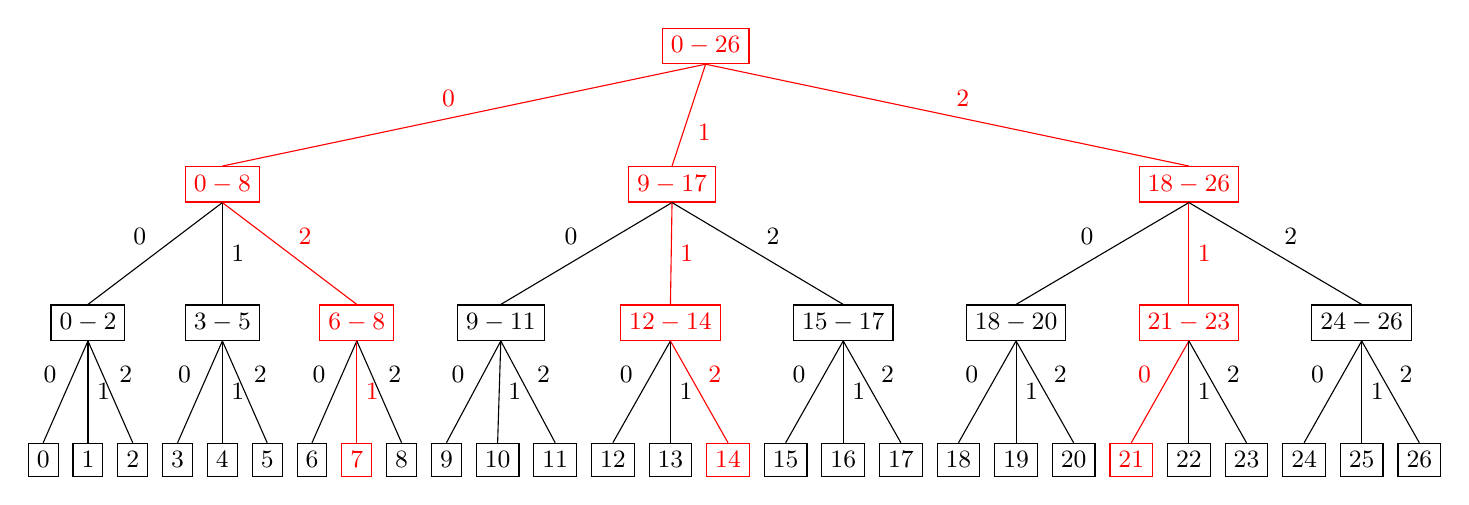
\begin{tikzpicture}[level distance=50pt, sibling distance=5pt]
\small
\Tree
[.\node[draw,red]{$0-26$}; 
	\edge[red] node[auto=right] {$0$};
	[.\node[draw,red]{$0-8$};
		\edge node[auto=right] {$0$};
		[.\node[draw]{$0-2$};
			\edge node[auto=right] {$0$};
			[.\node[draw]{$0$}; ]
			\edge node[auto=left] {$1$};
			[.\node[draw]{$1$}; ]
			\edge node[auto=left] {$2$};
			[.\node[draw]{$2$}; ] ]
		\edge node[auto=left] {$1$};
		[.\node[draw]{$3-5$};
			\edge node[auto=right] {$0$};
			[.\node[draw]{$3$}; ]
			\edge node[auto=left] {$1$};
			[.\node[draw]{$4$}; ]
			\edge node[auto=left] {$2$};
			[.\node[draw]{$5$}; ] ]
		\edge[red] node[auto=left] {$2$};
		[.\node[draw,red]{$6-8$};
			\edge node[auto=right] {$0$};
			[.\node[draw]{$6$}; ]
			\edge[red] node[auto=left] {$1$};
			[.\node[draw,red]{$7$}; ]
			\edge node[auto=left] {$2$};
			[.\node[draw]{$8$}; ] ] ]
	\edge[red] node[auto=left] {$1$};
	[.\node[draw,red]{$9-17$};
		\edge node[auto=right] {$0$};
		[.\node[draw]{$9-11$};
			\edge node[auto=right] {$0$};
			[.\node[draw]{$9$}; ]
			\edge node[auto=left] {$1$};
			[.\node[draw]{$10$}; ]
			\edge node[auto=left] {$2$};
			[.\node[draw]{$11$}; ] ]
		\edge[red] node[auto=left] {$1$};
		[.\node[draw,red]{$12-14$};
			\edge node[auto=right] {$0$};
			[.\node[draw]{$12$}; ]
			\edge node[auto=left] {$1$};
			[.\node[draw]{$13$}; ]
			\edge[red] node[auto=left] {$2$};
			[.\node[draw,red]{$14$}; ] ]
		\edge node[auto=left] {$2$};
		[.\node[draw]{$15-17$};
			\edge node[auto=right] {$0$};
			[.\node[draw]{$15$}; ]
			\edge node[auto=left] {$1$};
			[.\node[draw]{$16$}; ]
			\edge node[auto=left] {$2$};
			[.\node[draw]{$17$}; ] ] ]
	\edge[red] node[auto=left] {$2$};
	[.\node[draw,red]{$18-26$};
		\edge node[auto=right] {$0$};
		[.\node[draw]{$18-20$};
			\edge node[auto=right] {$0$};
			[.\node[draw]{$18$}; ]
			\edge node[auto=left] {$1$};
			[.\node[draw]{$19$}; ]
			\edge node[auto=left] {$2$};
			[.\node[draw]{$20$}; ] ]
		\edge[red] node[auto=left] {$1$};
		[.\node[draw,red]{$21-23$};
			\edge[red] node[auto=right] {$0$};
			[.\node[draw,red]{$21$}; ]
			\edge node[auto=left] {$1$};
			[.\node[draw]{$22$}; ]
			\edge node[auto=left] {$2$};
			[.\node[draw]{$23$}; ] ]
		\edge node[auto=left] {$2$};
		[.\node[draw]{$24-26$};
			\edge node[auto=right] {$0$};
			[.\node[draw]{$24$}; ]
			\edge node[auto=left] {$1$};
			[.\node[draw]{$25$}; ]
			\edge node[auto=left] {$2$};
			[.\node[draw]{$26$}; ] ] ]
		]
\end{tikzpicture}

Ez alapján a következő formula a becslések kiindulópontja. $f(p, k)$ a $k$. szinten a $p$ prímhez kapcsolódó műveletigény.
\begin{align*}
\sum_{k=0}^{m} \left( \sum_{p \le a^k} a^{m-k} f(p, k) + \sum_{a^k < p \le a^m} \frac{n}{p} f(p, k) \right)
\end{align*}

A második ötlet az optimális cache megfogása.
Ha a vödörműveletek konstans idejűek, az optimális cache algoritmus logikusnak tűnik. Mindig azokat a prím-pozíciókat kell tárolni a cache-ben, amik a leghamarabb fognak szitálni.
Azt már beláttam, hogy a kisebb vödörindexű párok hamarabb szitálnak, mint a nagyobb vödörindexűek. Egy egyszerű szimuláció megmutatja, hogy ez az algoritmus sokkal jobb, mint a legkisebb prímek tárolása a pozíciótól függetlenül.

Az optimális cache-sel a műveletigényt nem sikerült meghatároznom. Az ötletem az volt, hogy beszorítom a műveletigényét egy nem elég jó cache, és egy túl jó cache közé.
A nem elég jó cache a kis prímeket tároló cache.
A túl jó cache a fa alsó néhány szintjén mindent ingyenessé tesz, és a felsőbb szinteken minden egyes csúcsban a cache teljes méretével csökkenti a műveletigényt.
Ez annyira jó cache lenne, hogy meg se valósítható.

A probléma jó megfogalmazása itt is előjön, a cache méretét a következőképpen írtam le. Legyen  $c=a^d$, és a cache $\pi(c)$ db. prím-pozíció párt képes tárolni.

A képlet a következőképpen módosul a kis prímek cache-t figyelembe véve:
\begin{align*}
\sum_{k=0}^{m} \left( \sum_{ c < p \le a^k} a^{m-k} f(p, k) + \sum_{\max(c, a^k) < p \le a^m} \frac{n}{p} f(p, k) \right)
\end{align*}
A túl jó cache esetén:
\begin{align*}
\sum_{k=d+1}^{m} \left( \sum_{ p \le a^k} a^{m-k} f(p, k) + \sum_{a^k < p \le a^m} \frac{n}{p} f(p, k) - \text{amennyit csak meg lehet spórolni a cache-sel} \right)
\end{align*}

Szalagra írásnál a vödörműveletek műveletigénye nem konstans idejű.
Egyesével ki kell írni a prím számjegyeit, és a fában a levélig vezető út címkéit.
Azaz a $k$. szinten a $p$ prím kiírásának műveletigénye $k+\lceil\log_{a}(n)\rceil+1$.
A könnyebb számolás kedvéért ezt $k+\log_{a}(n)$-nek vettem.

A cache mérete számjegyekben $2m\pi(c)$ kell legyen, hogy bármelyik $\pi(c)$ db. prím-pozíciót képes legyen tárolni. A túl jó cache-nél ezt a műveletigényt veszem garantáltan megspóroltnak.

A szalag-modell másik problémája, hogy az optimális cache algoritmust nem ismerem.
Már az kérdés, hogy a párok számát, vagy a számjegyek számát vesszük a cache méretnek.
Ha a párok számát, akkor ugyanaz az optimális algoritmus, mint a konstans idős vödröknél, de nem lesz minden számjegy kihasználva.
Ha a számjegyek számát nézzük, akkor valószínűleg a cache-ben kihasznált számjegyek számának maximalizálása nem esik egybe a legközelebb szitáló párok kiválasztásával.

A sok-sok levezetésben igyekeztem az $R$-eknek elnevezett hibatagokat végigcipelni a számításon.
Egyrészt így nyugodtan egyenlőségjelet használhattam mindenhol.
Másrészt be lehetne fejezni a hibatagok becslését, amiből kiderülne, hogy mennyire pontos az eredmény.

\section{Felhasznált becslések}

A számrendszer alapja:
\begin{align*}
a \in \mathbb{N}^{+}, a > 1
\end{align*}

A szitált tartomány vége:
\begin{align*}
n = a^m, m \in \mathbb{N}^{+}
\end{align*}

A cache mérete, $\pi(c)$ prím+pozíció pár tárolható:
\begin{align*}
c = a^d, d \in \mathbb{N}_{0}, d < m
\end{align*}

Prímszámtétel, $n \ge 2$:
\begin{align*}
\pi(n) = \sum_{p \le n} 1 = \frac{n}{\ln{n}} + R_{\pi}(n)
\end{align*}

Mertens 1. tétele, $n \ge 2$:
\begin{align*}
\sum_{p \le n} \frac{\ln{p}}{p} = \ln{n} + R_1(n) \\
\lvert R_1(n) \rvert \le 2
\end{align*}

Mertens 2. tétele, $n \ge 2$:
\begin{align*}
\sum_{p \le n} \frac{1}{p} = \ln{\ln{n}} + M + R_2(n) \\
M \approx 0.261 \text{ (Meissel–Mertens konstans)} \\
\lvert R_2(n) \rvert \le \frac{4}{\ln{(n+1)}} + \frac{2}{n \ln{n}}
\end{align*}

Első Csebisev-függvény:
\begin{align*}
\vartheta(n) = \sum_{p \le n} \ln{p} = n + R_{\vartheta}(n) \\
R_{\vartheta}(n) \le 0.006788 \frac{n}{ln{n}} \text{ ha } n \ge 10544111
\end{align*}

Harmonikus sor, $n \ge 2$:
\begin{align*}
\sum_{k=1}^{n} \frac{1}{k} = \ln{n} + \gamma + R_h(n) \\
\gamma \approx 0.577 \text{ (Euler–Mascheroni konstans)} \\
R_h(n) \sim \frac{1}{2n}
\end{align*}

Geometrikus sor:
\begin{align*}
\sum_{k=0}^{n} \frac{1}{a^k}
= \frac{1}{a^n} \sum_{k=0}^{n} \frac{1}{a^{k-n}}
= \frac{1}{a^n} \sum_{k=0}^{n} a^{n-k}
= \frac{1}{a^n} \sum_{k=0}^{n} a^k
= \frac{a^{n+1}-1}{(a-1)a^n}
\end{align*}

Valamilyen-sor:
\begin{align*}
\sum_{k=1}^{n} \frac{k}{a^k}
=& \sum_{i=1}^{n} \sum_{k=i}^{n} \frac{1}{a^k}
= \sum_{i=1}^{n} \left( \sum_{k=0}^{n} \frac{1}{a^k} - \sum_{k=0}^{i-1} \frac{1}{a^k} \right) = \\
=& \sum_{i=1}^{n} \left( \frac{a^{n+1}-1}{(a-1)a^n} - \frac{a^{i}-1}{(a-1)a^{i-1}} \right) = \\
=& \sum_{i=1}^{n} \left( \frac{a^{n+1}-1}{(a-1)a^n} - \frac{a^{n+1}-a^{n-i+1}}{(a-1)a^{n}} \right) = \\
=& \sum_{i=1}^{n} \frac{a^{n-i+1}-1}{(a-1)a^n} = \\
=& \frac{1}{(a-1)a^n} \left( \sum_{i=1}^{n} a^{n-i+1} - \sum_{i=1}^{n} 1 \right) = \\
=& \frac{1}{(a-1)a^n} \left( \sum_{i=1}^{n} a^{i} - n \right) = \\
=& \frac{1}{(a-1)a^n} \left( \sum_{i=0}^{n} a^{i} - 1 - n \right) = \\
=& \frac{1}{(a-1)a^n} \left( \frac{a^{n+1}-1}{a-1} - 1 - n \right) = \\
=& \frac{1}{(a-1)a^n} \left( \frac{a^{n+1}-1}{a-1} - \frac{(1 + n)(a-1)}{a-1} \right) = \\
=& \frac{1}{(a-1)a^n} \left( \frac{a^{n+1}-1}{a-1} - \frac{a -1 +an -n}{a-1} \right) = \\
=& \frac{1}{(a-1)a^n} \frac{a^{n+1}-1-a+1-an+n}{a-1} = \\
=& \frac{a^{n+1} - a - a n + n}{(a-1)^2 a^n}
\end{align*}

Stirling-formula:
\begin{align*}
\sum_{k=1}^{n} \ln{k} = \ln{(n!)} = n \ln{n} - n + \frac{\ln{(2 \pi n)}}{2} + R_s(n)
\end{align*}

Euler-Maclaurin formula alapján:
\begin{align*}
\sum_{i=1}^{n} i \ln{i} = \frac{1}{2} n^2 \ln{n} - \frac{1}{4} n^2 + \frac{1}{2} n \ln{n} + \frac{1}{12} \ln{n} + \frac{1}{4} + R_{ll}(n) \\
\sum_{i=m+1}^{n} i \ln{i} = \frac{1}{2} n^2 \ln{n} - \frac{1}{4} n^2 + \frac{1}{2} n \ln{n} + \frac{1}{12} \ln{n} - \frac{1}{2} m^2 \ln{m} + \frac{1}{4} m^2 - \frac{1}{2} m \ln{m} - \frac{1}{12} \ln{m} + R_{lm}(m, n)
\end{align*}

$a^k$ nem prím:
\begin{align*}
\forall k \in \mathbb{N}_0 : \sum_{p \le a^k - 1} f(p) =\sum_{p \le a^k} f(p)
\end{align*}

\section{Konstans idejű vödörműveletek}

\subsection{Nincs cache}

\begin{align*}
C_0(n) =& \sum_{k=0}^{m} \left( a^{m-k} \pi(a^k) + \sum_{a^k < p \le a^m} \frac{n}{p} \right) = \\
=& \sum_{k=0}^{m} \left( a^{m-k} \pi(a^k) + n \sum_{a^k < p \le n} \frac{1}{p} \right) = \\
=& \sum_{k=0}^{m} \left( a^{m-k} \pi(a^k) + n \left( \sum_{p \le n} \frac{1}{p} - \sum_{p \le a^k} \frac{1}{p} \right) \right) = \\
=& n \sum_{p \le n} \frac{1}{p} + \sum_{k=1}^{m} \left( a^{m-k} \pi(a^k) + n \left( \sum_{p \le n} \frac{1}{p} - \sum_{p \le a^k} \frac{1}{p} \right) \right) \\
=& n \sum_{p \le n} \frac{1}{p} + \sum_{k=1}^{m} a^{m-k} \pi(a^k) + n \sum_{k=1}^{m} \left( \sum_{p \le n} \frac{1}{p} - \sum_{p \le a^k} \frac{1}{p} \right) = \\
=& C_{0,1}(n) + C_{0,2}(n) + C_{0,3}(n)
\end{align*}

\begin{align*}
C_{0,1}(n) =& n \sum_{p \le n} \frac{1}{p} = \\
=& n \left( \ln{\ln{n}} + M + R_2(n) \right) = \\
=& n \left( \ln{\ln{n}} + M \right) + R_{C_{0,1}}(n)
\end{align*}

\begin{align*}
C_{0,2}(n) =& \sum_{k=1}^{m} a^{m-k} \pi(a^k) = \\
=& \sum_{k=1}^{m} a^{m-k} \left( \frac{a^k}{\ln{a^k}} + R_{\pi}(a^k) \right) = \\
=& \sum_{k=1}^{m} \left( \frac{a^{m-k} a^k}{\ln{a^k}} + a^{m-k} R_{\pi}(a^k) \right) = \\
=& \sum_{k=1}^{m} \left( \frac{a^m}{\ln{a^k}} + a^{m-k} R_{\pi}(a^k) \right) = \\
=& \sum_{k=1}^{m} \left( \frac{n}{\ln{a^k}} + a^{m-k} R_{\pi}(a^k) \right) = \\
=& \sum_{k=1}^{m} \left( \frac{n}{k \ln{a}} + a^{m-k} R_{\pi}(a^k) \right) = \\
=& \sum_{k=1}^{m} \left( \frac{n}{k \ln{a}} + \frac{a^m}{a^k} R_{\pi}(a^k) \right) = \\
=& \sum_{k=1}^{m} \left( \frac{n}{k \ln{a}} + \frac{n}{a^k} R_{\pi}(a^k) \right) = \\
=& n \sum_{k=1}^{m} \left( \frac{1}{k \ln{a}} + \frac{R_{\pi}(a^k)}{a^k} \right) = \\
=& n \left( \sum_{k=1}^{m} \frac{1}{k \ln{a}} + \sum_{k=1}^{m} \frac{R_{\pi}(a^k)}{a^k} \right) = \\
=& n \left( \frac{1}{\ln{a}} \sum_{k=1}^{m} \frac{1}{k} + \sum_{k=1}^{m} \frac{R_{\pi}(a^k)}{a^k} \right) = \\
=& n \left( \frac{1}{\ln{a}} \left(  \ln{m} + \gamma + R_h(m) \right) + \sum_{k=1}^{m} \frac{R_{\pi}(a^k)}{a^k} \right) = \\
=& \frac{n( \ln{m} + \gamma )}{\ln{a}} + R_{C_{0,2}}(n) = \\
=& \frac{n( \ln{\frac{\ln{n}}{\ln{a}}} + \gamma )}{\ln{a}} + R_{C_{0,2}}(n) = \\
=& n \left( \frac{1}{\ln{a}}\ln{\frac{\ln{n}}{\ln{a}}} +  \frac{\gamma}{\ln{a}} \right) + R_{C_{0,2}}(n)
\end{align*}

\begin{align*}
C_{0,3}(n) =& n \sum_{k=1}^{m} \left( \sum_{p \le n} \frac{1}{p} - \sum_{p \le a^k} \frac{1}{p} \right) = \\
=& n \sum_{k=1}^{m} \left( \ln{\ln{n}} + M + R_2(n) - \ln{\ln{a^k}} - M - R_2(a^k) \right) = \\
=& n \sum_{k=1}^{m} \left( \ln{\ln{n}} - \ln{\ln{a^k}} + R_2(n) - R_2(a^k) \right) = \\
=& n \sum_{k=1}^{m} \left( \ln{\frac{\ln{n}}{\ln{a^k}}} + R_2(n) - R_2(a^k) \right) = \\
=& n \sum_{k=1}^{m} \left( \ln{\frac{\ln{a^m}}{\ln{a^k}}} + R_2(n) - R_2(a^k) \right) = \\
=& n \sum_{k=1}^{m} \left( \ln{\frac{m \ln{a}}{k \ln{a}}} + R_2(n) - R_2(a^k) \right) = \\
=& n \sum_{k=1}^{m} \left( \ln{\frac{m}{k}} + R_2(n) - R_2(a^k) \right) = \\
=& n \sum_{k=1}^{m} \left( \ln{m} - \ln{k} + R_2(n) - R_2(a^k) \right) = \\
=& n \left( \sum_{k=1}^{m} \ln{m} - \sum_{k=1}^{m} \ln{k} + \sum_{k=1}^{m} \left( R_2(n) - R_2(a^k) \right) \right) = \\
=& n \left( \ln{m} \sum_{k=1}^{m} 1 - \sum_{k=1}^{m} \ln{k} + \sum_{k=1}^{m} \left( R_2(n) - R_2(a^k) \right) \right) = \\
=& n \left( m \ln{m} - \sum_{k=1}^{m} \ln{k} + \sum_{k=1}^{m} \left( R_2(n) - R_2(a^k) \right) \right) = \\
=& n \left( m \ln{m} - \left( m \ln{m} - m + \frac{\ln{(2 \pi m)}}{2} + R_s(m) \right) + \sum_{k=1}^{m} \left( R_2(n) - R_2(a^k) \right) \right) = \\
=& n \left( m \ln{m} - m \ln{m} + m - \frac{\ln{(2 \pi m)}}{2} - R_s(m) + \sum_{k=1}^{m} \left( R_2(n) - R_2(a^k) \right) \right) = \\
=& n \left( m- \frac{\ln{(2 \pi m)}}{2} - R_s(m) + \sum_{k=1}^{m} \left( R_2(n) - R_2(a^k) \right) \right) = \\
=& n \left( m - \frac{\ln{(2 \pi m)}}{2} \right) + R_{C_{0,3}}(n)
\end{align*}

\begin{align*}
C_{0,3} =& n \left( m - \frac{\ln{(2 \pi) + \ln{m}}}{2} \right) + R_{C_{0,3}}(n) = \\
=& n \left( \frac{\ln{n}}{\ln{a}} - \frac{\ln{(2 \pi)} + \ln{\frac{\ln{n}}{\ln{a}}}}{2} \right) + R_{C_{0,3}}(n) = \\
=& n \left( \frac{\ln{n}}{\ln{a}} - \frac{\ln{(2 \pi)}}{2} - \frac{1}{2} \ln{\frac{\ln{n}}{\ln{a}}} \right) + R_{C_{0,3}}(n)
\end{align*}

\begin{align*}
C_0(n) =& C_{0,1}(n) + C_{0,2}(n) + C_{0,3}(n) = \\
=& n \left( \ln{\ln{n}} + M \right) + n \left( \frac{1}{\ln{a}}\ln{\frac{\ln{n}}{\ln{a}}} + \frac{\gamma}{\ln{a}} \right) + n \left( \frac{\ln{n}}{\ln{a}} - \frac{\ln{(2 \pi)}}{2} - \frac{1}{2} \ln{\frac{\ln{n}}{\ln{a}}} \right) + R_{C_0}(n) = \\
=& n \left( \ln{\ln{n}} + M + \frac{1}{\ln{a}}\ln{\frac{\ln{n}}{\ln{a}}} +  \frac{\gamma}{\ln{a}} + \frac{\ln{n}}{\ln{a}} - \frac{\ln{(2 \pi)}}{2} - \frac{1}{2} \ln{\frac{\ln{n}}{\ln{a}}} \right) + R_{C_0}(n) = \\
=& n \left(\frac{\ln{n}}{\ln{a}} + \ln{\ln{n}} + \frac{1}{\ln{a}}\ln{\frac{\ln{n}}{\ln{a}}} - \frac{1}{2} \ln{\frac{\ln{n}}{\ln{a}}} + \frac{\gamma}{\ln{a}} + M - \frac{\ln{(2 \pi)}}{2} \right) + R_{C_0}(n) = \\
=& n \left(\frac{\ln{n}}{\ln{a}} + \ln{\ln{n}} + \ln{\frac{\ln{n}}{\ln{a}}} \left( \frac{1}{\ln{a}} - \frac{1}{2} \right) + \frac{\gamma}{\ln{a}} + M - \frac{\ln{(2 \pi)}}{2} \right) + R_{C_0}(n)
\end{align*}

\subsection{Kis prímek cache}

\begin{align*}
C_K(n) =& \sum_{k=0}^{m} \left( a^{m-k} \max(0, \pi(a^k) - \pi(c) ) + \sum_{\max(a^k, c) < p \le a^m} \frac{n}{p} \right) = \\
=& \sum_{k=0}^{m} \left( a^{m-k} \max(0, \pi(a^k) - \pi(a^d) ) + \sum_{\max(a^k, a^d) < p \le a^m} \frac{n}{p} \right) = \\
=& \sum_{k=0}^{d} \sum_{a^d < p \le a^m} \frac{n}{p} + \sum_{k=d+1}^{m} \left( a^{m-k} ( \pi(a^k) - \pi(a^d) ) + \sum_{a^k < p \le a^m} \frac{n}{p} \right) = \\
=& \sum_{k=0}^{d} \sum_{a^d < p \le a^m} \frac{n}{p} + \sum_{k=d+1}^{m} a^{m-k} ( \pi(a^k) - \pi(a^d) ) + \sum_{k=d+1}^{m} \sum_{a^k < p \le a^m} \frac{n}{p} = \\
=& C_{K,1}(n) + C_{K,2}(n) + C_{K,3}(n)
\end{align*}

\begin{align*}
C_{K,1}(n) =& \sum_{k=0}^{d} \sum_{a^d < p \le a^m} \frac{n}{p} = \\
=& n \sum_{k=0}^{d} \sum_{a^d < p \le a^m} \frac{1}{p} = \\
=& n \left( d + 1 \right) \sum_{a^d < p \le a^m} \frac{1}{p} = \\
=& n \left( \frac{\ln{c}}{\ln{a}} + 1 \right) \sum_{c < p \le n} \frac{1}{p} = \\
=& n \left( \frac{\ln{c}}{\ln{a}} + 1 \right) \left( \sum_{p \le n} \frac{1}{p} - \sum_{p \le c} \frac{1}{p} \right) = \\
=& n \left( \frac{\ln{c}}{\ln{a}} + 1 \right) \left( \ln{\ln{n}} + M + R_2(n) - \ln{\ln{c}} - M - R_2(c) \right) = \\
=& n \left( \frac{\ln{c}}{\ln{a}} + 1 \right) \left( \ln{\ln{n}} - \ln{\ln{c}} + R_2(n) - R_2(c) \right) = \\
=& n \left( \frac{\ln{c}}{\ln{a}} + 1 \right) \left( \ln{\frac{\ln{n}}{\ln{c}}} + R_2(n) - R_2(c) \right) = \\
=& n \left( \frac{\ln{c}}{\ln{a}} + 1 \right) \ln{\frac{\ln{n}}{\ln{c}}} + R_{C_{K,1}}(n)
\end{align*}

\begin{align*}
C_{K,2}(n) =& \sum_{k=d+1}^{m} a^{m-k} \left( \pi(a^k) - \pi(a^d) \right) = \\
=& \sum_{k=d+1}^{m} a^{m-k} \left( \frac{a^k}{\ln{a^k}} + R_{\pi}(a^k) - \frac{a^d}{\ln{a^d}} - R_{\pi}(a^d) \right) = \\
=& \sum_{k=d+1}^{m} a^{m-k} \left( \frac{a^k}{k \ln{a}} - \frac{a^d}{d \ln{a}} + R_{\pi}(a^k) - R_{\pi}(a^d) \right) = \\
=& n \sum_{k=d+1}^{m} a^{-k} \left( \frac{a^k}{k \ln{a}} - \frac{a^d}{d \ln{a}} + R_{\pi}(a^k) - R_{\pi}(a^d) \right) = \\
=& n \sum_{k=d+1}^{m} \left( \frac{1}{k \ln{a}} - \frac{a^d}{d a^k \ln{a}} + \frac{R_{\pi}(a^k) - R_{\pi}(a^d)}{a^k} \right) = \\
=& n \left( \sum_{k=d+1}^{m} \frac{1}{k \ln{a}} - \sum_{k=d+1}^{m} \frac{a^d}{d a^k \ln{a}} + \sum_{k=d+1}^{m} \frac{R_{\pi}(a^k) - R_{\pi}(a^d)}{a^k} \right) = \\
=& \frac{n}{\ln{a}} \sum_{k=d+1}^{m} \frac{1}{k} - \frac{n a^d}{d \ln{a}} \sum_{k=d+1}^{m} \frac{1}{a^k} + n \sum_{k=d+1}^{m} \frac{R_{\pi}(a^k) - R_{\pi}(a^d)}{a^k} = \\
=& \frac{n}{\ln{a}} \sum_{k=d+1}^{m} \frac{1}{k} - \frac{n a^d}{d \ln{a}} \left( \sum_{k=0}^{m} \frac{1}{a^k} - \sum_{k=0}^{d} \frac{1}{a^k} \right) + n \sum_{k=d+1}^{m} \frac{R_{\pi}(a^k) - R_{\pi}(a^d)}{a^k} = \\
=& \frac{n}{\ln{a}} \sum_{k=d+1}^{m} \frac{1}{k} - \frac{n a^d}{d \ln{a}} \left( \frac{a^{m+1}-1}{(a-1)a^m} - \frac{a^{d+1}-1}{(a-1)a^d} \right) + n \sum_{k=d+1}^{m} \frac{R_{\pi}(a^k) - R_{\pi}(a^d)}{a^k} = \\
=& \frac{n}{\ln{a}} \sum_{k=d+1}^{m} \frac{1}{k} - \frac{n a^d}{d \ln{a}} \left( \frac{a^{m+1}-1}{(a-1)a^m} - \frac{a^{m+1}-a^{m-d}}{(a-1)a^m} \right) + n \sum_{k=d+1}^{m} \frac{R_{\pi}(a^k) - R_{\pi}(a^d)}{a^k} = \\
=& \frac{n}{\ln{a}} \sum_{k=d+1}^{m} \frac{1}{k} - \frac{n a^d}{d \ln{a}} \frac{a^{m+1}-1-a^{m+1}+a^{m-d}}{(a-1)a^m} + n \sum_{k=d+1}^{m} \frac{R_{\pi}(a^k) - R_{\pi}(a^d)}{a^k} = \\
=& \frac{n}{\ln{a}} \sum_{k=d+1}^{m} \frac{1}{k} - \frac{n a^d}{d \ln{a}} \frac{a^{m-d}-1}{(a-1)a^m} + n \sum_{k=d+1}^{m} \frac{R_{\pi}(a^k) - R_{\pi}(a^d)}{a^k} = \\
=& \frac{n}{\ln{a}} \sum_{k=d+1}^{m} \frac{1}{k} - \frac{n ( a^m - a^d )}{d (a-1) a^m \ln{a}} + n \sum_{k=d+1}^{m} \frac{R_{\pi}(a^k) - R_{\pi}(a^d)}{a^k} = \\
=& \frac{n}{\ln{a}} \sum_{k=d+1}^{m} \frac{1}{k} - \frac{n ( n - a^d )}{d (a-1) n \ln{a}} + n \sum_{k=d+1}^{m} \frac{R_{\pi}(a^k) - R_{\pi}(a^d)}{a^k} = \\
=& \frac{n}{\ln{a}} \sum_{k=d+1}^{m} \frac{1}{k} - \frac{n - a^d}{d (a-1) \ln{a}} + n \sum_{k=d+1}^{m} \frac{R_{\pi}(a^k) - R_{\pi}(a^d)}{a^k} = \\
\end{align*}

\begin{align*}
C_{K,2}(n)
=& \frac{n}{\ln{a}} \left( \sum_{k=1}^{m} \frac{1}{k} - \sum_{k=1}^{d} \frac{1}{k} \right) - \frac{n - a^d}{d (a-1) \ln{a}} + n \sum_{k=d+1}^{m} \frac{R_{\pi}(a^k) - R_{\pi}(a^d)}{a^k} = \\
=& \frac{n}{\ln{a}} \left( \ln{m} + \gamma + R_h(m) - \ln{d} - \gamma - R_h(d) \right) - \frac{n - a^d}{d (a-1) \ln{a}} + n \sum_{k=d+1}^{m} \frac{R_{\pi}(a^k) - R_{\pi}(a^d)}{a^k} = \\
=& \frac{n}{\ln{a}} \left( \ln{m} - \ln{d} + R_h(m) - R_h(d) \right) - \frac{n - a^d}{d (a-1) \ln{a}} + n \sum_{k=d+1}^{m} \frac{R_{\pi}(a^k) - R_{\pi}(a^d)}{a^k} = \\
=& \frac{n ( \ln{m} - \ln{d} )}{\ln{a}} - \frac{n - a^d}{d (a-1) \ln{a}} + R_{C_{K,2}}(n) = \\
=& \frac{n ( \ln{m} - \ln{d} )}{\ln{a}} - \frac{n - c}{\frac{\ln{c}}{\ln{a}} (a-1) \ln{a}} + R_{C_{K,2}}(n) = \\
=& \frac{n ( \ln{m} - \ln{d} )}{\ln{a}} - \frac{n - c}{\ln{c} (a-1)} + R_{C_{K,2}}(n) = \\
=& n \frac{1}{\ln{a}} \ln{\frac{m}{d}} - \frac{n - c}{\ln{c} (a-1)} + R_{C_{K,2}}(n) = \\
=& n \frac{1}{\ln{a}} \ln{\frac{\ln{n}}{\ln{c}}} - \frac{n - c}{\ln{c} (a-1)} + R_{C_{K,2}}(n)
\end{align*}

\begin{align*}
C_{K,3}(n) =& \sum_{k=d+1}^{m} \sum_{a^k < p \le a^m} \frac{n}{p} = \\
=& n \sum_{k=d+1}^{m} \sum_{a^k < p \le a^m} \frac{1}{p} = \\
=& n \sum_{k=d+1}^{m} \left( \sum_{p \le a^m} \frac{1}{p} - \sum_{p \le a^k} \frac{1}{p} \right) = \\
=& n \sum_{k=d+1}^{m} \left( \ln{\ln{a^m}} + M + R_2(a^m) - \ln{\ln{a^k}} - M - R_2(a^k) \right) = \\
=& n \sum_{k=d+1}^{m} \left( \ln{\ln{a^m}} - \ln{\ln{a^k}} + R_2(a^m) - R_2(a^k) \right) = \\
=& n \sum_{k=d+1}^{m} \left( \ln{\frac{\ln{a^m}}{\ln{a^k}}} + R_2(a^m) - R_2(a^k) \right) = \\
=& n \sum_{k=d+1}^{m} \left( \ln{\frac{m \ln{a}}{k \ln{a}}} + R_2(a^m) - R_2(a^k) \right) = \\
=& n \sum_{k=d+1}^{m} \left( \ln{\frac{m}{k}} + R_2(a^m) - R_2(a^k) \right) = \\
=& n \sum_{k=d+1}^{m} \left( \ln{m} - \ln{k} + R_2(a^m) - R_2(a^k) \right) = \\
=& n \left( \sum_{k=d+1}^{m} \ln{m} - \sum_{k=d+1}^{m} \ln{k} + \sum_{k=d+1}^{m} \left( R_2(a^m) - R_2(a^k) \right) \right) = \\
=& n \left( ( m - d ) \ln{m} - \sum_{k=d+1}^{m} \ln{k} + \sum_{k=d+1}^{m} \left( R_2(a^m) - R_2(a^k) \right) \right) = \\
=& n \left( ( m - d ) \ln{m} - \sum_{k=1}^{m} \ln{k} + \sum_{k=1}^{d} \ln{k} + \sum_{k=d+1}^{m} \left( R_2(a^m) - R_2(a^k) \right) \right) = \\
=& n \left( ( m - d ) \ln{m} - m \ln{m} + m - \frac{\ln{(2 \pi m)}}{2} - R_s(m) + d \ln{d} - d + \frac{\ln{(2 \pi d)}}{2} + R_s(d) + \sum_{k=d+1}^{m} \left( R_2(a^m) - R_2(a^k) \right) \right) = \\
=& n \left( ( m - d ) \ln{m} - m \ln{m} + m + d \ln{d} - d + \frac{\ln{(2 \pi d)}}{2} - \frac{\ln{(2 \pi m)}}{2} - R_s(m) + R_s(d) + \sum_{k=d+1}^{m} \left( R_2(a^m) - R_2(a^k) \right) \right) = \\
\end{align*}

\begin{align*}
C_{K,3}(n)
=& n \left( - d \ln{m} + m + d \ln{d} - d + \frac{\ln{(2 \pi d)}}{2} - \frac{\ln{(2 \pi m)}}{2} - R_s(m) + R_s(d) + \sum_{k=d+1}^{m} \left( R_2(a^m) - R_2(a^k) \right) \right) = \\
=& n \left( m - d - d ( \ln{m} - \ln{d} ) + \frac{\ln{(2 \pi d)} - \ln{(2 \pi m)}}{2} - R_s(m) + R_s(d) + \sum_{k=d+1}^{m} \left( R_2(a^m) - R_2(a^k) \right) \right) = \\
=& n \left( m - d - d ( \ln{m} - \ln{d} ) + \frac{\ln{(2 \pi)} + \ln{d} - \ln{(2 \pi)} - \ln{m}}{2} - R_s(m) + R_s(d) + \sum_{k=d+1}^{m} \left( R_2(a^m) - R_2(a^k) \right) \right) = \\
=& n \left( m - d - d ( \ln{m} - \ln{d} ) - \frac{\ln{m} - \ln{d}}{2} - R_s(m) + R_s(d) + \sum_{k=d+1}^{m} \left( R_2(a^m) - R_2(a^k) \right) \right) = \\
=& n \left( m - d - d ( \ln{m} - \ln{d} ) - \frac{\ln{m} - \ln{d}}{2} \right) + R_{C_{K,3}}(n) = \\
=& n \left( m - d - d \ln{\frac{m}{d}} - \frac{1}{2} \ln{\frac{m}{d}} \right) + R_{C_{K,3}}(n) = \\
=& n \left( m - d - \ln{\frac{m}{d}} \left( d + \frac{1}{2} \right) \right) + R_{C_{K,3}}(n) = \\
=& n \left( \frac{\ln{n}}{\ln{a}} - \frac{\ln{c}}{\ln{a}} - \ln{\frac{\ln{n}}{\ln{c}}} \left( \frac{\ln{c}}{\ln{a}} + \frac{1}{2} \right) \right) + R_{C_{K,3}}(n) = \\
=& n \left( \frac{1}{\ln{a}} \ln{\frac{n}{c}} - \ln{\frac{\ln{n}}{\ln{c}}} \left( \frac{\ln{c}}{\ln{a}} + \frac{1}{2} \right) \right) + R_{C_{K,3}}(n)
\end{align*}

\begin{align*}
C_K(n) =& C_{K,1}(n) + C_{K,2}(n) + C_{K,3}(n) = \\
=& n \left( \frac{\ln{c}}{\ln{a}} + 1 \right) \ln{\frac{\ln{n}}{\ln{c}}} + n \frac{1}{\ln{a}} \ln{\frac{\ln{n}}{\ln{c}}} - \frac{n - c}{\ln{c} (a-1)} + n \left( \frac{1}{\ln{a}} \ln{\frac{n}{c}} - \ln{\frac{\ln{n}}{\ln{c}}} \left( \frac{\ln{c}}{\ln{a}} + \frac{1}{2} \right) \right) + R_{C_K}(n) = \\
=& n \left( \frac{1}{\ln{a}} \ln{\frac{n}{c}} + \left( \frac{\ln{c}}{\ln{a}} + 1 \right) \ln{\frac{\ln{n}}{\ln{c}}} + \frac{1}{\ln{a}} \ln{\frac{\ln{n}}{\ln{c}}} - \ln{\frac{\ln{n}}{\ln{c}}} \left( \frac{\ln{c}}{\ln{a}} + \frac{1}{2} \right)  \right) - \frac{n - c}{\ln{c} (a-1)} + R_{C_K}(n) = \\
=& n \left( \frac{1}{\ln{a}} \ln{\frac{n}{c}} + \left( \frac{\ln{c}}{\ln{a}} + 1 + \frac{1}{\ln{a}} - \frac{\ln{c}}{\ln{a}} - \frac{1}{2} \right) \ln{\frac{\ln{n}}{\ln{c}}}  \right) - \frac{n - c}{\ln{c} (a-1)} + R_{C_K}(n) = \\
=& n \left( \frac{1}{\ln{a}} \ln{\frac{n}{c}} + \left( \frac{1}{\ln{a}} + \frac{1}{2} \right) \ln{\frac{\ln{n}}{\ln{c}}}  \right) - \frac{n - c}{\ln{c} (a-1)} + R_{C_K}(n)
\end{align*}

\subsection{Túl jó cache}

\begin{align*}
C_T(n) =& \sum_{k=d+1}^{m} a^{m-k} \left( \pi(a^k) + \sum_{a^k < p \le a^m} \frac{a^k}{p} - \pi(a^d) \right) = \\
=& \sum_{k=d+1}^{m} a^{m-k} \left( \pi(a^k) - \pi(a^d) \right) + \sum_{k=d+1}^{m} \sum_{a^k < p \le a^m} \frac{n}{p} = \\
=& C_{K,2}(n) + C_{K,3}(n) = \\
=& n \frac{1}{\ln{a}} \ln{\frac{\ln{n}}{\ln{c}}} - \frac{n - c}{\ln{c} (a-1)} + n \left( \frac{1}{\ln{a}} \ln{\frac{n}{c}} - \ln{\frac{\ln{n}}{\ln{c}}} \left( \frac{\ln{c}}{\ln{a}} + \frac{1}{2} \right) \right) + R_{C_T}(n) = \\
=& n \left( \frac{1}{\ln{a}} \ln{\frac{n}{c}} + \frac{1}{\ln{a}} \ln{\frac{\ln{n}}{\ln{c}}} - \ln{\frac{\ln{n}}{\ln{c}}} \left( \frac{\ln{c}}{\ln{a}} + \frac{1}{2} \right) \right) - \frac{n - c}{\ln{c} (a-1)} + R_{C_T}(n) = \\
=& n \left( \frac{1}{\ln{a}} \ln{\frac{n}{c}} + \ln{\frac{\ln{n}}{ \ln{c}}} \left( \frac{1}{\ln{a}} - \frac{\ln{c}}{\ln{a}} - \frac{1}{2} \right) \right) - \frac{n - c}{\ln{c} (a-1)} + R_{C_T}(n)
\end{align*}

\subsection{Optimális cache}

\begin{align*}
C_K(n)- C_{OPT}(n) < C_K(n)- C_T(n) = C_{K,1}(n) = n \left( \frac{\ln{c}}{\ln{a}} + 1 \right) \ln{\frac{\ln{n}}{\ln{c}}} + R_{C_{K,1}}(n)
\end{align*}

\section{Szalag-vödör}

\subsection{Nincs cache}

\begin{align*}
L_0(n) =& \sum_{k=0}^{m} \left( a^{m-k} \sum_{p \le a^k} \left( k + \frac{\ln{p}}{\ln{a}} \right) + \sum_{a^k < p \le a^m} \frac{n}{p} \left( k + \frac{\ln{p}}{\ln{a}} \right) \right) = \\
=& \sum_{k=0}^{m} \left( k a^{m-k} \sum_{p \le a^k} 1 + \frac{a^{m-k}}{\ln{a}} \sum_{p \le a^k} \ln{p} + n k \sum_{a^k < p \le a^m} \frac{1}{p} + \frac{n}{\ln{a}} \sum_{a^k < p \le a^m} \frac{\ln{p}}{p} \right) = \\
=& \sum_{k=0}^{m} k a^{m-k} \sum_{p \le a^k} 1 + \sum_{k=0}^{m} \frac{a^{m-k}}{\ln{a}} \sum_{p \le a^k} \ln{p} + \sum_{k=0}^{m} n k \sum_{a^k < p \le a^m} \frac{1}{p} + \sum_{k=0}^{m} \frac{n}{\ln{a}} \sum_{a^k < p \le a^m} \frac{\ln{p}}{p} = \\
=& n \sum_{k=0}^{m} \frac{k}{a^k} \sum_{p \le a^k} 1 + \frac{n}{\ln{a}} \sum_{k=0}^{m} \frac{1}{a^k} \sum_{p \le a^k} \ln{p} + n \sum_{k=0}^{m} k \sum_{a^k < p \le a^m} \frac{1}{p} + \frac{n}{\ln{a}} \sum_{k=0}^{m} \sum_{a^k < p \le a^m} \frac{\ln{p}}{p} = \\
=& L_{0,1}(n) + L_{0,2}(n) + L_{0,3}(n) + L_{0,4}(n)
\end{align*}

\begin{align*}
L_{0,1}(n) =& n \sum_{k=0}^{m} \frac{k}{a^k} \sum_{p \le a^k} 1 = \\
=& n \sum_{k=0}^{m} \frac{k}{a^k} \left( \frac{a^k}{\ln{a^k}} + R_{\pi}(n) \right) = \\
=& n \sum_{k=0}^{m} \frac{k}{a^k} \frac{a^k}{\ln{a^k}} + n \sum_{k=0}^{m} \frac{k}{a^k} R_{\pi}(n) = \\
=& n \sum_{k=0}^{m} \frac{k}{\ln{a^k}} + n \sum_{k=0}^{m} \frac{k}{a^k} R_{\pi}(n) = \\
=& n \sum_{k=0}^{m} \frac{k}{k \ln{a}} + n \sum_{k=0}^{m} \frac{k}{a^k} R_{\pi}(n) = \\
=& n \sum_{k=0}^{m} \frac{1}{\ln{a}} + n \sum_{k=0}^{m} \frac{k}{a^k} R_{\pi}(n) = \\
=& \frac{n}{\ln{a}} \sum_{k=0}^{m} 1 + n \sum_{k=0}^{m} \frac{k}{a^k} R_{\pi}(n) = \\
=& \frac{n}{\ln{a}} \left( 1 + m \right) + n \sum_{k=0}^{m} \frac{k}{a^k} R_{\pi}(n) = \\
=& \frac{n}{\ln{a}} \left( 1 + \frac{\ln{n}}{\ln{a}} \right) + n \sum_{k=0}^{m} \frac{k}{a^k} R_{\pi}(n) = \\
=& n \left( \frac{1}{\ln{a}} + \frac{\ln{n}}{\ln^2{a}} \right) + n \sum_{k=0}^{m} \frac{k}{a^k} R_{\pi}(n) = \\
=& n \left( \frac{1}{\ln{a}} + \frac{1}{\ln^2{a}} \ln{n} \right) + R_{L_{0,1}}(n) \\
\end{align*}

\begin{align*}
L_{0,2}(n) =& \frac{n}{\ln{a}} \sum_{k=0}^{m} \frac{1}{a^k} \sum_{p \le a^k} \ln{p} = \\
=& \frac{n}{\ln{a}} \sum_{k=0}^{m} \frac{1}{a^k} \left( a^k + R_{\vartheta}(a^k) \right) = \\
=& \frac{n}{\ln{a}} \sum_{k=0}^{m} \frac{1}{a^k} a^k + \frac{n}{\ln{a}} \sum_{k=0}^{m} \frac{1}{a^k} R_{\vartheta}(a^k) = \\
=& \frac{n}{\ln{a}} \sum_{k=0}^{m} 1 + \frac{n}{\ln{a}} \sum_{k=0}^{m} \frac{1}{a^k} R_{\vartheta}(a^k) = \\
=& \frac{n}{\ln{a}} \left( 1 + m \right) + \frac{n}{\ln{a}} \sum_{k=0}^{m} \frac{1}{a^k} R_{\vartheta}(a^k) = \\
=& \frac{n}{\ln{a}} \left( 1 + \frac{\ln{n}}{\ln{a}} \right) + \frac{n}{\ln{a}} \sum_{k=0}^{m} \frac{1}{a^k} R_{\vartheta}(a^k) = \\
=& n \left( \frac{1}{\ln{a}} + \frac{\ln{n}}{\ln^2{a}} \right) + \frac{n}{\ln{a}} \sum_{k=0}^{m} \frac{1}{a^k} R_{\vartheta}(a^k) = \\
=& n \left( \frac{1}{\ln{a}} + \frac{1}{\ln^2{a}} \ln{n} \right) + R_{L_{0,2}}(n)
\end{align*}

\begin{align*}
L_{0,3}(n) =& n \sum_{k=0}^{m} k \sum_{a^k < p \le a^m} \frac{1}{p} = \\
=& n \sum_{k=1}^{m} k \sum_{a^k < p \le a^m} \frac{1}{p} = \\
=& n \sum_{k=1}^{m} k \left( \sum_{p \le a^m} \frac{1}{p} - \sum_{p \le a^k} \frac{1}{p} \right) = \\
=& n \sum_{k=1}^{m} k \left( \ln{\ln{a^m}} + M + R_2(a^m) - \ln{\ln{a^k}} - M - R_2(a^k) \right) = \\
=& n \sum_{k=1}^{m} k \left( \ln{\ln{a^m}} - \ln{\ln{a^k}} + R_2(a^m) - R_2(a^k) \right) = \\
=& n \sum_{k=1}^{m} k \left( \ln{\frac{\ln{a^m}}{\ln{a^k}}} + R_2(a^m) - R_2(a^k) \right) = \\
=& n \sum_{k=1}^{m} k \left( \ln{\frac{m \ln{a}}{k \ln{a}}} + R_2(a^m) - R_2(a^k) \right) = \\
=& n \sum_{k=1}^{m} k \left( \ln{\frac{m}{k}} + R_2(a^m) - R_2(a^k) \right) = \\
=& n \sum_{k=1}^{m} k \left( \ln{m} - \ln{k} + R_2(a^m) - R_2(a^k) \right) = \\
=& n \left( \sum_{k=1}^{m} k \ln{m} - \sum_{k=1}^{m} k \ln{k} \right) + n \sum_{k=1}^{m} k \left( R_2(a^m) - R_2(a^k) \right) = \\
=& n \left( \ln{m} \sum_{k=1}^{m} k - \sum_{k=1}^{m} k \ln{k} \right) + n \sum_{k=1}^{m} k \left( R_2(a^m) - R_2(a^k) \right) = \\
=& n \left( \frac{1}{2} m (1 + m) \ln{m} - \sum_{k=1}^{m} k \ln{k} \right) + n \sum_{k=1}^{m} k \left( R_2(a^m) - R_2(a^k) \right) = \\
=& n \left( \frac{1}{2} m (1 + m) \ln{m} - \frac{1}{2} m^2 \ln{m} + \frac{1}{4} m^2 - \frac{1}{2} m \ln{m} - \frac{1}{12} \ln{m} - \frac{1}{4} - R_{ll}(m) \right) + n \sum_{k=1}^{m} k \left( R_2(a^m) - R_2(a^k) \right) = \\
=& n \left( \frac{1}{2} m \ln{m} + \frac{1}{4} m^2 - \frac{1}{2} m \ln{m} - \frac{1}{12} \ln{m} - \frac{1}{4} - R_{ll}(m) \right) + n \sum_{k=1}^{m} k \left( R_2(a^m) - R_2(a^k) \right) = \\
=& n \left( \frac{1}{4} m^2 - \frac{1}{12} \ln{m} - \frac{1}{4} - R_{ll}(m) \right) + n \sum_{k=1}^{m} k \left( R_2(a^m) - R_2(a^k) \right) = L_{0,3}(n)
\end{align*}

\begin{align*}
L_{0,3}(n) =& n \left( \frac{1}{4} m^2 - \frac{1}{12} \ln{m} - \frac{1}{4} \right) + n \left(  - R_{ll}(m) + \sum_{k=1}^{m} k \left( R_2(a^m) - R_2(a^k) \right) \right) = \\
=& n \left( \frac{1}{4 \ln^2{a}} \ln^2{n} - \frac{1}{12} \ln{\frac{\ln{n}}{\ln{a}}} - \frac{1}{4} \right) + n \left(  - R_{ll}(m) + \sum_{k=1}^{m} k \left( R_2(a^m) - R_2(a^k) \right) \right) = \\
=& n \left( \frac{1}{4 \ln^2{a}} \ln^2{n} - \frac{1}{12} \ln{\frac{\ln{n}}{\ln{a}}} - \frac{1}{4} \right) + R_{L_{0,3}}(n)
\end{align*}

\begin{align*}
L_{0,4}(n) =& \frac{n}{\ln{a}} \sum_{k=0}^{m} \sum_{a^k < p \le a^m} \frac{\ln{p}}{p} = \\
=& \frac{n}{\ln{a}} \sum_{k=0}^{m} \left( \sum_{p \le a^m} \frac{\ln{p}}{p} - \sum_{p \le a^k} \frac{\ln{p}}{p} \right) = \\
=& \frac{n}{\ln{a}} \sum_{k=0}^{m} \left( \ln{a^m} + R_1(a^m) - \ln{a^k} - R_1(a^k) \right) = \\
=& n \left( \frac{1}{\ln{a}} \sum_{k=0}^{m} \ln{a^m} - \frac{1}{\ln{a}} \sum_{k=0}^{m} \ln{a^k} \right) + \frac{n}{\ln{a}} \sum_{k=0}^{m} \left( R_1(a^m) - R_1(a^k) \right) = \\
=& n \left( \frac{1}{\ln{a}} \sum_{k=0}^{m} \ln{n} - \frac{1}{\ln{a}} \sum_{k=0}^{m} k \ln{a} \right) + \frac{n}{\ln{a}} \sum_{k=0}^{m} \left( R_1(a^m) - R_1(a^k) \right) = \\
=& n \left( \frac{\ln{n}}{\ln{a}} \sum_{k=0}^{m} 1 - \sum_{k=0}^{m} k \right) + \frac{n}{\ln{a}} \sum_{k=0}^{m} \left( R_1(a^m) - R_1(a^k) \right) = \\
=& n \left( \frac{\ln{n}}{\ln{a}} \left( 1 + m \right) - \frac{1}{2} m \left( 1 + m \right) \right) + \frac{n}{\ln{a}} \sum_{k=0}^{m} \left( R_1(a^m) - R_1(a^k) \right) = \\
=& n \left( \frac{\ln{n}}{\ln{a}} \left( 1 + \frac{\ln{n}}{\ln{a}} \right) - \frac{1}{2} \frac{\ln{n}}{\ln{a}} \left( 1 + \frac{\ln{n}}{\ln{a}} \right) \right) + \frac{n}{\ln{a}} \sum_{k=0}^{m} \left( R_1(a^m) - R_1(a^k) \right) = \\
=& n \left( \frac{\ln{n}}{\ln{a}} + \frac{\ln^2{n}}{\ln^2{a}} - \frac{1}{2} \frac{\ln{n}}{\ln{a}} - \frac{1}{2} \frac{\ln^2{n}}{\ln^2{a}} \right) + \frac{n}{\ln{a}} \sum_{k=0}^{m} \left( R_1(a^m) - R_1(a^k) \right) = \\
=& n \left( \frac{1}{2} \frac{\ln^2{n}}{\ln^2{a}} + \frac{1}{2} \frac{\ln{n}}{\ln{a}} \right) + \frac{n}{\ln{a}} \sum_{k=0}^{m} \left( R_1(a^m) - R_1(a^k) \right) = \\
=& n \left( \frac{1}{2 \ln^2{a}} \ln^2{n} + \frac{1}{2 \ln{a}} \ln{n} \right) + R_{L_{0,4}}(n)
\end{align*}

\begin{align*}
L_{0}(n) =& L_{0,1}(n) + L_{0,2}(n) + L_{0,3}(n) + L_{0,4}(n) = \\
=& n \left( \frac{1}{\ln{a}} + \frac{1}{\ln^2{a}} \ln{n} + \frac{1}{\ln{a}} + \frac{1}{\ln^2{a}} \ln{n} + \frac{1}{4 \ln^2{a}} \ln^2{n} - \frac{1}{12} \ln{\frac{\ln{n}}{\ln{a}}} - \frac{1}{4} + \frac{1}{2 \ln^2{a}} \ln^2{n} + \frac{1}{2 \ln{a}} \ln{n} \right) + R_{L_{0}}(n) = \\
=& n \left( \frac{3}{4 \ln^2{a}} \ln^2{n} + \left( \frac{2}{\ln^2{a}} + \frac{1}{2 \ln{a}} \right) \ln{n} - \frac{1}{12} \ln{\frac{\ln{n}}{\ln{a}}} + \frac{2}{\ln{a}} - \frac{1}{4} \right) + R_{L_{0}}(n)
\end{align*}

\subsection{Kis prímek cache}

\begin{align*}
L_K(n) =& \sum_{k=0}^{m} \left( a^{m-k} \sum_{a^d < p \le a^k} \left( k + \frac{\ln{p}}{\ln{a}} \right) + \sum_{\max(a^d, a^k) < p \le a^m} \frac{n}{p} \left( k + \frac{\ln{p}}{\ln{a}} \right) \right) = \\
=& \sum_{k=0}^{d} \sum_{a^d < p \le a^m} \frac{n}{p} \left( k + \frac{\ln{p}}{\ln{a}} \right) + \sum_{k=d+1}^{m} \left( a^{m-k} \sum_{a^d < p \le a^k} \left( k + \frac{\ln{p}}{\ln{a}} \right) + \sum_{a^k < p \le a^m} \frac{n}{p} \left( k + \frac{\ln{p}}{\ln{a}} \right) \right) = \\
=& \sum_{k=0}^{d} \sum_{a^d < p \le a^m} \frac{n}{p} \left( k + \frac{\ln{p}}{\ln{a}} \right) + \sum_{k=d+1}^{m} a^{m-k} \sum_{a^d < p \le a^k} \left( k + \frac{\ln{p}}{\ln{a}} \right) + \sum_{k=d+1}^{m} \sum_{a^k < p \le a^m} \frac{n}{p} \left( k + \frac{\ln{p}}{\ln{a}} \right) = \\
=& L_{K,1}(n) +  L_{K,2}(n) +  L_{K,3}(n)
\end{align*}

\begin{align*}
L_{K,1}(n) =& \sum_{k=0}^{d} \sum_{a^d < p \le a^m} \frac{n}{p} \left( k + \frac{\ln{p}}{\ln{a}} \right) = \\
=& \sum_{k=0}^{d} \sum_{a^d < p \le a^m} \frac{n}{p} k + \sum_{k=0}^{d} \sum_{a^d < p \le a^m} \frac{n}{p} \frac{\ln{p}}{\ln{a}} = \\
=& n \sum_{k=0}^{d} k \sum_{a^d < p \le a^m} \frac{1}{p} + \frac{n}{\ln{a}} \sum_{k=0}^{d} \sum_{a^d < p \le a^m} \frac{\ln{p}}{p} = \\
=& n \sum_{k=0}^{d} k \sum_{a^d < p \le a^m} \frac{1}{p} + \frac{n \left( 1 + d \right)}{\ln{a}} \sum_{a^d < p \le a^m} \frac{\ln{p}}{p} = \\
=& n \sum_{k=0}^{d} k \sum_{a^d < p \le a^m} \frac{1}{p} + \frac{n \left( 1 + d \right)}{\ln{a}} \left( \sum_{p \le a^m} \frac{\ln{p}}{p} - \sum_{p \le a^d} \frac{\ln{p}}{p} \right) = \\
=& n \sum_{k=0}^{d} k \sum_{a^d < p \le a^m} \frac{1}{p} + \frac{n \left( 1 + d \right)}{\ln{a}} \left( \ln{a^m} + R_1(a^m) - \ln{a^d} - R_1(a^d) \right) = \\
=& n \sum_{k=0}^{d} k \sum_{a^d < p \le a^m} \frac{1}{p} + \frac{n \left( 1 + d \right)}{\ln{a}} \left( \ln{a^m} - \ln{a^d} + R_1(a^m) - R_1(a^d) \right) = \\
=& n \sum_{k=0}^{d} k \sum_{a^d < p \le a^m} \frac{1}{p} + \frac{n \left( 1 + d \right)}{\ln{a}} \left( \ln{a^m} - \ln{a^d} \right) + \frac{n \left( 1 + d \right)}{\ln{a}} \left( R_1(a^m) - R_1(a^d) \right) = \\
=& n \sum_{k=0}^{d} k \sum_{a^d < p \le a^m} \frac{1}{p} + \frac{n \left( 1 + d \right)}{\ln{a}} \left( m \ln{a} - d \ln{a} \right) + \frac{n \left( 1 + d \right)}{\ln{a}} \left( R_1(a^m) - R_1(a^d) \right) = \\
=& n \sum_{k=0}^{d} k \sum_{a^d < p \le a^m} \frac{1}{p} + n \left( 1 + d \right) \left( m - d \right) + \frac{n \left( 1 + d \right)}{\ln{a}} \left( R_1(a^m) - R_1(a^d) \right) = \\
=& n \left( \sum_{a^d < p \le a^m} \frac{1}{p} \right) \sum_{k=0}^{d} k + n \left( 1 + d \right) \left( m - d \right) + \frac{n \left( 1 + d \right)}{\ln{a}} \left( R_1(a^m) - R_1(a^d) \right) = \\
=& \frac{n d ( 1 + d )}{2} \left( \sum_{a^d < p \le a^m} \frac{1}{p} \right) + n \left( 1 + d \right) \left( m - d \right) + \frac{n \left( 1 + d \right)}{\ln{a}} \left( R_1(a^m) - R_1(a^d) \right) = \\
=& \frac{n d ( 1 + d )}{2} \left( \sum_{p \le a^m} \frac{1}{p} - \sum_{p \le a^d} \frac{1}{p} \right) + n \left( 1 + d \right) \left( m - d \right) + \frac{n \left( 1 + d \right)}{\ln{a}} \left( R_1(a^m) - R_1(a^d) \right) = \\
\end{align*}

\begin{align*}
L_{K,1}(n) =& \frac{n d ( 1 + d )}{2} \left( \ln{\ln{a^m}} + M + R_2(a^m) - \ln{\ln{a^d}} - M - R_2(a^d) \right) + n \left( 1 + d \right) \left( m - d \right) + \frac{n \left( 1 + d \right)}{\ln{a}} \left( R_1(a^m) - R_1(a^d) \right) = \\
=& \frac{n d ( 1 + d )}{2} \left( \ln{\ln{a^m}} - \ln{\ln{a^d}} + R_2(a^m) - R_2(a^d) \right) + n \left( 1 + d \right) \left( m - d \right) + \frac{n \left( 1 + d \right)}{\ln{a}} \left( R_1(a^m) - R_1(a^d) \right) = \\
=& \frac{n d ( 1 + d )}{2} \left( \ln{\ln{a^m}} - \ln{\ln{a^d}} \right) + \frac{n d ( 1 + d )}{2} \left( R_2(a^m) - R_2(a^d) \right) + n \left( 1 + d \right) \left( m - d \right) + \frac{n \left( 1 + d \right)}{\ln{a}} \left( R_1(a^m) - R_1(a^d) \right) = \\
=& \frac{n d ( 1 + d )}{2} \left( \ln{\ln{a^m}} - \ln{\ln{a^d}} \right) + n \left( 1 + d \right) \left( m - d \right) + \frac{n d ( 1 + d )}{2} \left( R_2(a^m) - R_2(a^d) \right) + \frac{n \left( 1 + d \right)}{\ln{a}} \left( R_1(a^m) - R_1(a^d) \right) = \\
=& \frac{n d ( 1 + d )}{2} \ln{\frac{\ln{a^m}}{\ln{a^d}}} + n \left( 1 + d \right) \left( m - d \right) + \frac{n d ( 1 + d )}{2} \left( R_2(a^m) - R_2(a^d) \right) + \frac{n \left( 1 + d \right)}{\ln{a}} \left( R_1(a^m) - R_1(a^d) \right) = \\
=& \frac{n d ( 1 + d )}{2} \ln{\frac{m \ln{a}}{d \ln{a}}} + n \left( 1 + d \right) \left( m - d \right) + \frac{n d ( 1 + d )}{2} \left( R_2(a^m) - R_2(a^d) \right) + \frac{n \left( 1 + d \right)}{\ln{a}} \left( R_1(a^m) - R_1(a^d) \right) = \\
=& \frac{n d ( 1 + d )}{2} \ln{\frac{m}{d}} + n \left( 1 + d \right) \left( m - d \right) + \frac{n d ( 1 + d )}{2} \left( R_2(a^m) - R_2(a^d) \right) + \frac{n \left( 1 + d \right)}{\ln{a}} \left( R_1(a^m) - R_1(a^d) \right) = \\
=& \frac{n d ( 1 + d )}{2} \ln{\frac{m}{d}} + n \left( 1 + d \right) \left( m - d \right) + R_{L_{K,1}}(n) = \\
=& n \left( \frac{1}{2} d ( 1 + d ) \ln{\frac{m}{d}} + \left( 1 + d \right) \left( m - d \right) \right) + R_{L_{K,1}}(n) = \\
=& n \left( \frac{1}{2} \frac{\ln{c}}{\ln{a}} \left( 1 + \frac{\ln{c}}{\ln{a}} \right) \ln{\frac{\frac{\ln{n}}{\ln{a}}}{\frac{\ln{c}}{\ln{a}}}} + \left( 1 + \frac{\ln{c}}{\ln{a}} \right) \left( \frac{\ln{n}}{\ln{a}} - \frac{\ln{c}}{\ln{a}} \right) \right) + R_{L_{K,1}}(n) = \\
=& n \left( \frac{\ln{c}}{2\ln{a}} \left( 1 + \frac{\ln{c}}{\ln{a}} \right) \ln{\frac{\ln{n}}{\ln{c}}} + \frac{1}{\ln{a}} \left( 1 + \frac{\ln{c}}{\ln{a}} \right) \left( \ln{n} - \ln{c} \right) \right) + R_{L_{K,1}}(n) = \\
=& n \left( \frac{\ln{c}}{2\ln{a}} \left( 1 + \frac{\ln{c}}{\ln{a}} \right) \ln{\frac{\ln{n}}{\ln{c}}} + \frac{1}{\ln{a}} \left( 1 + \frac{\ln{c}}{\ln{a}} \right) \ln{\frac{n}{c}} \right) + R_{L_{K,1}}(n) = \\
=& n \left( \frac{1}{\ln{a}} \left( 1 + \frac{\ln{c}}{\ln{a}} \right) \ln{\frac{n}{c}} + \frac{\ln{c}}{2\ln{a}} \left( 1 + \frac{\ln{c}}{\ln{a}} \right) \ln{\frac{\ln{n}}{\ln{c}}} \right) + R_{L_{K,1}}(n)
\end{align*}

\begin{align*}
L_{K,2}(n) =& \sum_{k=d+1}^{m} a^{m-k} \sum_{a^d < p \le a^k} \left( k + \frac{\ln{p}}{\ln{a}} \right) = \\
=& n \sum_{k=d+1}^{m} \frac{1}{a^k} \sum_{a^d < p \le a^k} \left( k + \frac{\ln{p}}{\ln{a}} \right) = \\
=& n \left( \sum_{k=d+1}^{m} \frac{1}{a^k} \sum_{a^d < p \le a^k} k + \sum_{k=d+1}^{m} \frac{1}{a^k} \sum_{a^d < p \le a^k} \frac{\ln{p}}{\ln{a}} \right) = \\
=& n \left( \sum_{k=d+1}^{m} \frac{k}{a^k} \sum_{a^d < p \le a^k} 1 + \frac{1}{\ln{a}} \sum_{k=d+1}^{m} \frac{1}{a^k} \sum_{a^d < p \le a^k} \ln{p} \right) = \\
=& n \left( \sum_{k=d+1}^{m} \frac{k}{a^k} \sum_{a^d < p \le a^k} 1 + \frac{1}{\ln{a}} \sum_{k=d+1}^{m} \frac{1}{a^k} \left( \sum_{p \le a^k} \ln{p} - \sum_{p \le a^d} \ln{p} \right) \right) = \\
=& n \left( \sum_{k=d+1}^{m} \frac{k}{a^k} \sum_{a^d < p \le a^k} 1 + \frac{1}{\ln{a}} \sum_{k=d+1}^{m} \frac{1}{a^k} \left( a^k + R_{\vartheta}(a^k) - a^d - R_{\vartheta}(a^d) \right) \right) = \\
=& n \left( \sum_{k=d+1}^{m} \frac{k}{a^k} \sum_{a^d < p \le a^k} 1 + \frac{1}{\ln{a}} \sum_{k=d+1}^{m} \frac{1}{a^k} a^k - \frac{1}{\ln{a}}\sum_{k=d+1}^{m} \frac{1}{a^k} a^d + \frac{1}{\ln{a}} \sum_{k=d+1}^{m} \frac{1}{a^k} \left( R_{\vartheta}(a^k) - R_{\vartheta}(a^d) \right) \right) = \\
=& n \left( \sum_{k=d+1}^{m} \frac{k}{a^k} \sum_{a^d < p \le a^k} 1 + \frac{1}{\ln{a}} \sum_{k=d+1}^{m} 1 - \frac{a^d}{\ln{a}} \sum_{k=d+1}^{m} \frac{1}{a^k} + \frac{1}{\ln{a}} \sum_{k=d+1}^{m} \frac{1}{a^k} \left( R_{\vartheta}(a^k) - R_{\vartheta}(a^d) \right) \right) = \\
=& n \left( \sum_{k=d+1}^{m} \frac{k}{a^k} \sum_{a^d < p \le a^k} 1 + \frac{1}{\ln{a}} \left( m - d \right) - \frac{a^d}{\ln{a}} \sum_{k=d+1}^{m} \frac{1}{a^k} + \frac{1}{\ln{a}} \sum_{k=d+1}^{m} \frac{1}{a^k} \left( R_{\vartheta}(a^k) - R_{\vartheta}(a^d) \right) \right) = \\
=& n \left( \sum_{k=d+1}^{m} \frac{k}{a^k} \sum_{a^d < p \le a^k} 1 + \frac{1}{\ln{a}} \left( m - d \right) - \frac{a^d}{\ln{a}} \left( \sum_{k=0}^{m} \frac{1}{a^k} - \sum_{k=0}^{d} \frac{1}{a^k} \right) + \frac{1}{\ln{a}} \sum_{k=d+1}^{m} \frac{1}{a^k} \left( R_{\vartheta}(a^k) - R_{\vartheta}(a^d) \right) \right) = \\
=& n \left( \sum_{k=d+1}^{m} \frac{k}{a^k} \sum_{a^d < p \le a^k} 1 + \frac{1}{\ln{a}} \left( m - d \right) - \frac{a^d}{\ln{a}} \left( \frac{a^{m+1}-1}{(a-1)a^m} - \frac{a^{d+1}-1}{(a-1)a^d} \right) + \frac{1}{\ln{a}} \sum_{k=d+1}^{m} \frac{1}{a^k} \left( R_{\vartheta}(a^k) - R_{\vartheta}(a^d) \right) \right) = \\
=& n \left( \sum_{k=d+1}^{m} \frac{k}{a^k} \sum_{a^d < p \le a^k} 1 + \frac{1}{\ln{a}} \left( m - d \right) - \frac{a^d}{\ln{a}} \left( \frac{a^{m+1}-1}{(a-1)a^m} - \frac{a^{m+1}-a^{m-d}}{(a-1)a^m} \right) + \frac{1}{\ln{a}} \sum_{k=d+1}^{m} \frac{1}{a^k} \left( R_{\vartheta}(a^k) - R_{\vartheta}(a^d) \right) \right) = \\
=& n \left( \sum_{k=d+1}^{m} \frac{k}{a^k} \sum_{a^d < p \le a^k} 1 + \frac{1}{\ln{a}} \left( m - d \right) - \frac{a^d}{\ln{a}} \frac{a^{m-d}-1}{(a-1)a^m} + \frac{1}{\ln{a}} \sum_{k=d+1}^{m} \frac{1}{a^k} \left( R_{\vartheta}(a^k) - R_{\vartheta}(a^d) \right) \right) =
\end{align*}

\begin{align*}
L_{K,2}(n) =& n \left( \sum_{k=d+1}^{m} \frac{k}{a^k} \sum_{a^d < p \le a^k} 1 + \frac{1}{\ln{a}} \left( m - d \right) - \frac{a^m - a^d}{(a-1)a^m\ln{a}} + \frac{1}{\ln{a}} \sum_{k=d+1}^{m} \frac{1}{a^k} \left( R_{\vartheta}(a^k) - R_{\vartheta}(a^d) \right) \right) = \\
=& n \left( \sum_{k=d+1}^{m} \frac{k}{a^k} \left( \sum_{p \le a^k} 1 - \sum_{p \le a^d} 1 \right) + \frac{1}{\ln{a}} \left( m - d \right) - \frac{a^m - a^d}{(a-1)a^m\ln{a}} + \frac{1}{\ln{a}} \sum_{k=d+1}^{m} \frac{1}{a^k} \left( R_{\vartheta}(a^k) - R_{\vartheta}(a^d) \right) \right) = \\
=& n \left( \sum_{k=d+1}^{m} \frac{k}{a^k} \left( \frac{a^k}{\ln{a^k}} + R_{\pi}(a^k) - \frac{a^d}{\ln{a^d}} - R_{\pi}(a^d) \right) + \frac{1}{\ln{a}} \left( m - d \right) - \frac{a^m - a^d}{(a-1)a^m\ln{a}} + \frac{1}{\ln{a}} \sum_{k=d+1}^{m} \frac{1}{a^k} \left( R_{\vartheta}(a^k) - R_{\vartheta}(a^d) \right) \right) = \\
=& n \left( \sum_{k=d+1}^{m} \frac{k}{a^k} \left( \frac{a^k}{\ln{a^k}} - \frac{a^d}{\ln{a^d}} \right) + \frac{1}{\ln{a}} \left( m - d \right) - \frac{a^m - a^d}{(a-1)a^m\ln{a}} + \sum_{k=d+1}^{m} \frac{k}{a^k} \left( R_{\pi}(a^k) - R_{\pi}(a^d) \right) + \frac{1}{\ln{a}} \sum_{k=d+1}^{m} \frac{1}{a^k} \left( R_{\vartheta}(a^k) - R_{\vartheta}(a^d) \right) \right) = \\
=& n \left( \sum_{k=d+1}^{m} \frac{k}{a^k} \left( \frac{a^k}{k \ln{a}} - \frac{a^d}{d \ln{a}} \right) + \frac{1}{\ln{a}} \left( m - d \right) - \frac{a^m - a^d}{(a-1)a^m\ln{a}} + \sum_{k=d+1}^{m} \frac{k}{a^k} \left( R_{\pi}(a^k) - R_{\pi}(a^d) \right) + \frac{1}{\ln{a}} \sum_{k=d+1}^{m} \frac{1}{a^k} \left( R_{\vartheta}(a^k) - R_{\vartheta}(a^d) \right) \right) = \\
=& n \left( \sum_{k=d+1}^{m} \frac{k}{a^k} \frac{a^k}{k \ln{a}} - \sum_{k=d+1}^{m} \frac{k}{a^k} \frac{a^d}{d \ln{a}} + \frac{1}{\ln{a}} \left( m - d \right) - \frac{a^m - a^d}{(a-1)a^m\ln{a}} + \sum_{k=d+1}^{m} \frac{k}{a^k} \left( R_{\pi}(a^k) - R_{\pi}(a^d) \right) + \frac{1}{\ln{a}} \sum_{k=d+1}^{m} \frac{1}{a^k} \left( R_{\vartheta}(a^k) - R_{\vartheta}(a^d) \right) \right) = \\
=& n \left( \sum_{k=d+1}^{m} \frac{1}{\ln{a}} - \sum_{k=d+1}^{m} \frac{k}{a^k} \frac{a^d}{d \ln{a}} + \frac{1}{\ln{a}} \left( m - d \right) - \frac{a^m - a^d}{(a-1)a^m\ln{a}} + \sum_{k=d+1}^{m} \frac{k}{a^k} \left( R_{\pi}(a^k) - R_{\pi}(a^d) \right) + \frac{1}{\ln{a}} \sum_{k=d+1}^{m} \frac{1}{a^k} \left( R_{\vartheta}(a^k) - R_{\vartheta}(a^d) \right) \right) = \\
=& n \left( \frac{1}{\ln{a}} \left( m - d \right) - \sum_{k=d+1}^{m} \frac{k}{a^k} \frac{a^d}{d \ln{a}} + \frac{1}{\ln{a}} \left( m - d \right) - \frac{a^m - a^d}{(a-1)a^m\ln{a}} + \sum_{k=d+1}^{m} \frac{k}{a^k} \left( R_{\pi}(a^k) - R_{\pi}(a^d) \right) + \frac{1}{\ln{a}} \sum_{k=d+1}^{m} \frac{1}{a^k} \left( R_{\vartheta}(a^k) - R_{\vartheta}(a^d) \right) \right) = \\
=& n \left( \frac{2}{\ln{a}} \left( m - d \right) - \sum_{k=d+1}^{m} \frac{k}{a^k} \frac{a^d}{d \ln{a}} - \frac{a^m - a^d}{(a-1)a^m\ln{a}} + \sum_{k=d+1}^{m} \frac{k}{a^k} \left( R_{\pi}(a^k) - R_{\pi}(a^d) \right) + \frac{1}{\ln{a}} \sum_{k=d+1}^{m} \frac{1}{a^k} \left( R_{\vartheta}(a^k) - R_{\vartheta}(a^d) \right) \right) = \\
=& n \left( \frac{2}{\ln{a}} \left( m - d \right) - \frac{a^d}{d \ln{a}} \sum_{k=d+1}^{m} \frac{k}{a^k} - \frac{a^m - a^d}{(a-1)a^m\ln{a}} + \sum_{k=d+1}^{m} \frac{k}{a^k} \left( R_{\pi}(a^k) - R_{\pi}(a^d) \right) + \frac{1}{\ln{a}} \sum_{k=d+1}^{m} \frac{1}{a^k} \left( R_{\vartheta}(a^k) - R_{\vartheta}(a^d) \right) \right) = \\
=& n \left( \frac{2}{\ln{a}} \left( m - d \right) - \frac{a^d}{d \ln{a}} \left( \sum_{k=1}^{m} \frac{k}{a^k} - \sum_{k=1}^{d} \frac{k}{a^k} \right) - \frac{a^m - a^d}{(a-1)a^m\ln{a}} + \sum_{k=d+1}^{m} \frac{k}{a^k} \left( R_{\pi}(a^k) - R_{\pi}(a^d) \right) + \frac{1}{\ln{a}} \sum_{k=d+1}^{m} \frac{1}{a^k} \left( R_{\vartheta}(a^k) - R_{\vartheta}(a^d) \right) \right) = \\
=& n \left( \frac{2}{\ln{a}} \left( m - d \right) - \frac{a^d}{d \ln{a}} \left( \frac{a^{m+1} - a - a m + m}{(a-1)^2 a^m} - \frac{a^{m+1} - a^{m - d + 1} - d a^{m - d + 1} + d a^{m-d}}{(a-1)^2 a^m} \right) - \frac{a^m - a^d}{(a-1)a^m\ln{a}} + \sum_{k=d+1}^{m} \frac{k}{a^k} \left( R_{\pi}(a^k) - R_{\pi}(a^d) \right) + \frac{1}{\ln{a}} \sum_{k=d+1}^{m} \frac{1}{a^k} \left( R_{\vartheta}(a^k) - R_{\vartheta}(a^d) \right) \right) = \\
=& n \left( \frac{2}{\ln{a}} \left( m - d \right) - \frac{a^d}{d \ln{a}} \left( \frac{a^{m+1} - a - a m + m - a^{m+1} + a^{m - d + 1} + d a^{m - d + 1} - d a^{m-d}}{(a-1)^2 a^m} \right) - \frac{a^m - a^d}{(a-1)a^m\ln{a}} + \sum_{k=d+1}^{m} \frac{k}{a^k} \left( R_{\pi}(a^k) - R_{\pi}(a^d) \right) + \frac{1}{\ln{a}} \sum_{k=d+1}^{m} \frac{1}{a^k} \left( R_{\vartheta}(a^k) - R_{\vartheta}(a^d) \right) \right) = \\
=& n \left( \frac{2}{\ln{a}} \left( m - d \right) - \frac{a^d}{d \ln{a}} \frac{- a - a m + m + a^{m - d + 1} + d a^{m - d + 1} - d a^{m-d}}{(a-1)^2 a^m} - \frac{a^m - a^d}{(a-1)a^m\ln{a}} + \sum_{k=d+1}^{m} \frac{k}{a^k} \left( R_{\pi}(a^k) - R_{\pi}(a^d) \right) + \frac{1}{\ln{a}} \sum_{k=d+1}^{m} \frac{1}{a^k} \left( R_{\vartheta}(a^k) - R_{\vartheta}(a^d) \right) \right) =
\end{align*}

\begin{align*}
L_{K,2}(n) =& n \left( \frac{2}{\ln{a}} \left( m - d \right) - \frac{- a^{d+1} - m a^{d+1} + m a^d + a^{m + 1} + d a^{m + 1} - d a^{m}}{d (a-1)^2 a^m \ln{a}} - \frac{a^m - a^d}{(a-1)a^m\ln{a}} + \sum_{k=d+1}^{m} \frac{k}{a^k} \left( R_{\pi}(a^k) - R_{\pi}(a^d) \right) + \frac{1}{\ln{a}} \sum_{k=d+1}^{m} \frac{1}{a^k} \left( R_{\vartheta}(a^k) - R_{\vartheta}(a^d) \right) \right) = \\
=& n \left( \frac{2}{\ln{a}} \left( m - d \right) - \frac{a^d ( - a - m a + m ) + a^m ( a + d a - d)}{d (a-1)^2 a^m \ln{a}} - \frac{a^m - a^d}{(a-1)a^m\ln{a}} + \sum_{k=d+1}^{m} \frac{k}{a^k} \left( R_{\pi}(a^k) - R_{\pi}(a^d) \right) + \frac{1}{\ln{a}} \sum_{k=d+1}^{m} \frac{1}{a^k} \left( R_{\vartheta}(a^k) - R_{\vartheta}(a^d) \right) \right) = \\
=& n \left( \frac{2}{\ln{a}} \left( m - d \right) - \frac{a^d ( - a - m a + m )}{d (a-1)^2 a^m \ln{a}} - \frac{a^m ( a + d a - d)}{d (a-1)^2 a^m \ln{a}} - \frac{a^m - a^d}{(a-1)a^m\ln{a}} + \sum_{k=d+1}^{m} \frac{k}{a^k} \left( R_{\pi}(a^k) - R_{\pi}(a^d) \right) + \frac{1}{\ln{a}} \sum_{k=d+1}^{m} \frac{1}{a^k} \left( R_{\vartheta}(a^k) - R_{\vartheta}(a^d) \right) \right) = \\
=& n \left( \frac{2}{\ln{a}} \left( m - d \right) + \frac{a^d ( a + m a - m )}{d (a-1)^2 a^m \ln{a}} - \frac{ a + d a - d}{d (a-1)^2 \ln{a}} - \frac{a^m - a^d}{(a-1)a^m\ln{a}} + \sum_{k=d+1}^{m} \frac{k}{a^k} \left( R_{\pi}(a^k) - R_{\pi}(a^d) \right) + \frac{1}{\ln{a}} \sum_{k=d+1}^{m} \frac{1}{a^k} \left( R_{\vartheta}(a^k) - R_{\vartheta}(a^d) \right) \right) = \\
=& n \left( \frac{2}{\ln{a}} \left( m - d \right) + \frac{c ( a + m a - m )}{d (a-1)^2 n \ln{a}} - \frac{ a + d a - d}{d (a-1)^2 \ln{a}} - \frac{n - c}{(a-1)n\ln{a}} + \sum_{k=d+1}^{m} \frac{k}{a^k} \left( R_{\pi}(a^k) - R_{\pi}(a^d) \right) + \frac{1}{\ln{a}} \sum_{k=d+1}^{m} \frac{1}{a^k} \left( R_{\vartheta}(a^k) - R_{\vartheta}(a^d) \right) \right) = \\
=& n \left( \frac{2}{\ln{a}} \left( m - d \right) + \frac{c ( a + m a - m )}{d (a-1)^2 n \ln{a}} - \frac{ a + d a - d}{d (a-1)^2 \ln{a}} - \frac{n - c}{(a-1)n\ln{a}} \right) + R_{L_{K,2}}(n) = \\
=& n \left( \frac{2}{\ln{a}} \left( m - d \right) - \frac{a + d a - d}{d (a-1)^2 \ln{a}} \right) - \frac{n - c}{(a-1) \ln{a}} + \frac{c ( a + m a - m )}{d (a-1)^2 \ln{a}} + R_{L_{K,2}}(n) = \\
=& n \left( \frac{2}{\ln{a}} \left( m - d \right) - \frac{a + d ( a - 1 )}{d (a-1)^2 \ln{a}} \right) - \frac{n - c}{(a-1) \ln{a}} + \frac{c ( a + m ( a - 1 ) )}{d (a-1)^2 \ln{a}} + R_{L_{K,2}}(n) = \\
=& n \left( \frac{2}{\ln{a}} \left( m - d \right) - \frac{a}{d (a-1)^2 \ln{a}} - \frac{ d ( a - 1 )}{d (a-1)^2 \ln{a}} \right) - \frac{n - c}{(a-1) \ln{a}} + \frac{c a}{d (a-1)^2 \ln{a}} + \frac{c m ( a - 1 )}{d (a-1)^2 \ln{a}} + R_{L_{K,2}}(n) = \\
=& n \left( \frac{2}{\ln{a}} \left( m - d \right) - \frac{a}{d (a-1)^2 \ln{a}} - \frac{1}{(a-1) \ln{a}} \right) - \frac{n - c}{(a-1) \ln{a}} + \frac{c a}{d (a-1)^2 \ln{a}} + \frac{c m}{d (a-1) \ln{a}} + R_{L_{K,2}}(n) = \\
=& n \left( \frac{2}{\ln{a}} \left( \frac{\ln{n}}{\ln{a}} - \frac{\ln{c}}{\ln{a}} \right) - \frac{a}{\frac{\ln{c}}{\ln{a}} (a-1)^2 \ln{a}} - \frac{1}{(a-1) \ln{a}} \right) - \frac{n - c}{(a-1) \ln{a}} + \frac{c a}{\frac{\ln{c}}{\ln{a}} (a-1)^2 \ln{a}} + \frac{c \frac{\ln{n}}{\ln{a}}}{\frac{\ln{c}}{\ln{a}} (a-1) \ln{a}} + R_{L_{K,2}}(n) = \\
=& n \left( \frac{2}{\ln^2{a}} \ln{\frac{n}{c}} - \frac{a}{\ln{c} (a-1)^2} - \frac{1}{(a-1) \ln{a}} \right) - \frac{n - c}{(a-1) \ln{a}} + \frac{c a}{\ln{c} (a-1)^2} + \frac{c}{\ln{c} (a-1) \ln{a}} \ln{n} + R_{L_{K,2}}(n)
\end{align*}

\begin{align*}
L_{K,3}(n) =& \sum_{k=d+1}^{m} \sum_{a^k < p \le a^m} \frac{n}{p} \left( k + \frac{\ln{p}}{\ln{a}} \right) = \\
=& n \sum_{k=d+1}^{m} \left( \sum_{a^k < p \le a^m} \frac{1}{p} k + \sum_{a^k < p \le a^m} \frac{1}{p} \frac{\ln{p}}{\ln{a}} \right) = \\
=& n \sum_{k=d+1}^{m} \left( k \sum_{a^k < p \le a^m} \frac{1}{p} + \frac{1}{\ln{a}} \sum_{a^k < p \le a^m} \frac{\ln{p}}{p} \right) = \\
=& n \left( \sum_{k=d+1}^{m} k \sum_{a^k < p \le a^m} \frac{1}{p} + \frac{1}{\ln{a}} \sum_{k=d+1}^{m} \sum_{a^k < p \le a^m} \frac{\ln{p}}{p} \right) = \\
=& n \left( \sum_{k=d+1}^{m} k \sum_{a^k < p \le a^m} \frac{1}{p} + \frac{1}{\ln{a}} \sum_{k=d+1}^{m} \left( \sum_{p \le a^m} \frac{\ln{p}}{p} - \sum_{p \le a^k} \frac{\ln{p}}{p} \right) \right) = \\
=& n \left( \sum_{k=d+1}^{m} k \sum_{a^k < p \le a^m} \frac{1}{p} + \frac{1}{\ln{a}} \sum_{k=d+1}^{m} \left( \ln{a^m} + R_1(a^m) - \ln{a^k} - R_1(a^k) \right) \right) = \\
=& n \left( \sum_{k=d+1}^{m} k \sum_{a^k < p \le a^m} \frac{1}{p} + \frac{1}{\ln{a}} \sum_{k=d+1}^{m} \left( \ln{a^m} - \ln{a^k} \right) + \frac{1}{\ln{a}} \sum_{k=d+1}^{m} \left( R_1(a^m) - R_1(a^k) \right) \right) = \\
=& n \left( \sum_{k=d+1}^{m} k \sum_{a^k < p \le a^m} \frac{1}{p} + \frac{1}{\ln{a}} \sum_{k=d+1}^{m} \left( m \ln{a} - k \ln{a} \right) + \frac{1}{\ln{a}} \sum_{k=d+1}^{m} \left( R_1(a^m) - R_1(a^k) \right) \right) = \\
=& n \left( \sum_{k=d+1}^{m} k \sum_{a^k < p \le a^m} \frac{1}{p} + \sum_{k=d+1}^{m} \left( m - k \right) + \frac{1}{\ln{a}} \sum_{k=d+1}^{m} \left( R_1(a^m) - R_1(a^k) \right) \right) = \\
=& n \left( \sum_{k=d+1}^{m} k \sum_{a^k < p \le a^m} \frac{1}{p} + \sum_{k=d+1}^{m} m - \sum_{k=d+1}^{m} k + \frac{1}{\ln{a}} \sum_{k=d+1}^{m} \left( R_1(a^m) - R_1(a^k) \right) \right) = \\
=& n \left( \sum_{k=d+1}^{m} k \sum_{a^k < p \le a^m} \frac{1}{p} + m ( m - d ) - \frac{1}{2} ( m - d ) ( m + d + 1 ) + \frac{1}{\ln{a}} \sum_{k=d+1}^{m} \left( R_1(a^m) - R_1(a^k) \right) \right) = \\
=& n \left( \sum_{k=d+1}^{m} k \sum_{a^k < p \le a^m} \frac{1}{p} + m^2 - d m + \frac{1}{2} ( d - m  ) ( m + d + 1 ) + \frac{1}{\ln{a}} \sum_{k=d+1}^{m} \left( R_1(a^m) - R_1(a^k) \right) \right) = \\
=& n \left( \sum_{k=d+1}^{m} k \sum_{a^k < p \le a^m} \frac{1}{p} + m^2 - d m + \frac{1}{2} ( d m + d^2 + d - m^2 - dm - m ) + \frac{1}{\ln{a}} \sum_{k=d+1}^{m} \left( R_1(a^m) - R_1(a^k) \right) \right) = \\
=& n \left( \sum_{k=d+1}^{m} k \sum_{a^k < p \le a^m} \frac{1}{p} + m^2 - d m + \frac{1}{2} (  d^2 + d - m^2 - m ) + \frac{1}{\ln{a}} \sum_{k=d+1}^{m} \left( R_1(a^m) - R_1(a^k) \right) \right) = \\
=& n \left( \sum_{k=d+1}^{m} k \sum_{a^k < p \le a^m} \frac{1}{p} + \frac{1}{2} (  d^2 + d + m^2 - m - 2 d m ) + \frac{1}{\ln{a}} \sum_{k=d+1}^{m} \left( R_1(a^m) - R_1(a^k) \right) \right) = \\
=& n \left( \sum_{k=d+1}^{m} k \left( \sum_{p \le a^m} \frac{1}{p} - \sum_{p \le a^k} \frac{1}{p} \right) + \frac{1}{2} (  d^2 + d + m^2 - m - 2 d m ) + \frac{1}{\ln{a}} \sum_{k=d+1}^{m} \left( R_1(a^m) - R_1(a^k) \right) \right) = \\
=& n \left( \sum_{k=d+1}^{m} k \left( \ln{\ln{a^m}} + M + R_2(a^m) - \ln{\ln{a^k}} - M - R_2(a^k) \right) + \frac{1}{2} (  d^2 + d + m^2 - m - 2 d m ) + \frac{1}{\ln{a}} \sum_{k=d+1}^{m} \left( R_1(a^m) - R_1(a^k) \right) \right) = \\
=& n \left( \sum_{k=d+1}^{m} k \left( \ln{\ln{a^m}} - \ln{\ln{a^k}} \right) + \frac{1}{2} (  d^2 + d + m^2 - m - 2 d m ) + \sum_{k=d+1}^{m} k \left( R_2(a^m) - R_2(a^k) \right) + \frac{1}{\ln{a}} \sum_{k=d+1}^{m} \left( R_1(a^m) - R_1(a^k) \right) \right) = \\
=& n \left( \sum_{k=d+1}^{m} k \left( \ln{\frac{\ln{a^m}}{\ln{a^k}}} \right) + \frac{1}{2} (  d^2 + d + m^2 - m - 2 d m ) + \sum_{k=d+1}^{m} k \left( R_2(a^m) - R_2(a^k) \right) + \frac{1}{\ln{a}} \sum_{k=d+1}^{m} \left( R_1(a^m) - R_1(a^k) \right) \right) =
\end{align*}

\begin{align*}
L_{K,3}(n) =& n \left( \sum_{k=d+1}^{m} k \left( \ln{\frac{m \ln{a}}{k \ln{a}}} \right) + \frac{1}{2} (  d^2 + d + m^2 - m - 2 d m ) + \sum_{k=d+1}^{m} k \left( R_2(a^m) - R_2(a^k) \right) + \frac{1}{\ln{a}} \sum_{k=d+1}^{m} \left( R_1(a^m) - R_1(a^k) \right) \right) = \\
=& n \left( \sum_{k=d+1}^{m} k \left( \ln{\frac{m}{k}} \right) + \frac{1}{2} (  d^2 + d + m^2 - m - 2 d m ) + \sum_{k=d+1}^{m} k \left( R_2(a^m) - R_2(a^k) \right) + \frac{1}{\ln{a}} \sum_{k=d+1}^{m} \left( R_1(a^m) - R_1(a^k) \right) \right) = \\
=& n \left( \sum_{k=d+1}^{m} k \ln{m} - \sum_{k=d+1}^{m} k \ln{k} + \frac{1}{2} (  d^2 + d + m^2 - m - 2 d m ) + \sum_{k=d+1}^{m} k \left( R_2(a^m) - R_2(a^k) \right) + \frac{1}{\ln{a}} \sum_{k=d+1}^{m} \left( R_1(a^m) - R_1(a^k) \right) \right) = \\
=& n \left( \ln{m} \sum_{k=d+1}^{m} k - \sum_{k=d+1}^{m} k \ln{k} + \frac{1}{2} (  d^2 + d + m^2 - m - 2 d m ) + \sum_{k=d+1}^{m} k \left( R_2(a^m) - R_2(a^k) \right) + \frac{1}{\ln{a}} \sum_{k=d+1}^{m} \left( R_1(a^m) - R_1(a^k) \right) \right) = \\
=& n \left( \frac{1}{2} ( m - d ) ( m + d + 1 ) \ln{m} - \sum_{k=d+1}^{m} k \ln{k} + \frac{1}{2} (  d^2 + d + m^2 - m - 2 d m ) + \sum_{k=d+1}^{m} k \left( R_2(a^m) - R_2(a^k) \right) + \frac{1}{\ln{a}} \sum_{k=d+1}^{m} \left( R_1(a^m) - R_1(a^k) \right) \right) = \\
=& n \left( \frac{1}{2} ( m^2 + d m + m - d m - d^2 - d ) \ln{m} - \sum_{k=d+1}^{m} k \ln{k} + \frac{1}{2} (  d^2 + d + m^2 - m - 2 d m ) + \sum_{k=d+1}^{m} k \left( R_2(a^m) - R_2(a^k) \right) + \frac{1}{\ln{a}} \sum_{k=d+1}^{m} \left( R_1(a^m) - R_1(a^k) \right) \right) = \\
=& n \left( \frac{1}{2} ( m^2 + m - d^2 - d ) \ln{m} - \sum_{k=d+1}^{m} k \ln{k} + \frac{1}{2} (  d^2 + d + m^2 - m - 2 d m ) + \sum_{k=d+1}^{m} k \left( R_2(a^m) - R_2(a^k) \right) + \frac{1}{\ln{a}} \sum_{k=d+1}^{m} \left( R_1(a^m) - R_1(a^k) \right) \right) = \\
=& n \left( \frac{1}{2} ( m^2 + m - d^2 - d ) \ln{m} + \frac{1}{2} (  d^2 + d + m^2 - m - 2 d m ) \right) - \\
-& n \left( \sum_{k=d+1}^{m} k \ln{k} \right) + \\
+& n \left( \sum_{k=d+1}^{m} k \left( R_2(a^m) - R_2(a^k) \right) + \frac{1}{\ln{a}} \sum_{k=d+1}^{m} \left( R_1(a^m) - R_1(a^k) \right) \right) = \\
=& n \left( \frac{1}{2} ( m^2 + m - d^2 - d ) \ln{m} + \frac{1}{2} (  d^2 + d + m^2 - m - 2 d m ) \right) - \\
-& n \left( \frac{1}{2} m^2 \ln{m} - \frac{1}{4} m^2 + \frac{1}{2} m \ln{m} + \frac{1}{12} \ln{m} - \frac{1}{2} d^2 \ln{d} + \frac{1}{4} d^2 - \frac{1}{2} d \ln{d} - \frac{1}{12} \ln{d} + R_{lm}(d, n) \right) + \\
+& n \left( \sum_{k=d+1}^{m} k \left( R_2(a^m) - R_2(a^k) \right) + \frac{1}{\ln{a}} \sum_{k=d+1}^{m} \left( R_1(a^m) - R_1(a^k) \right) \right) = \\
=& n \left( \frac{1}{2} m^2 \ln{m} + \frac{1}{2} m \ln{m} - \frac{1}{2} d^2 \ln{m} - \frac{1}{2} d \ln{m} + \frac{1}{2} d^2 + \frac{1}{2} d + \frac{1}{2} m^2 - \frac{1}{2} m - d m \right) + \\
+& n \left( - \frac{1}{2} m^2 \ln{m} + \frac{1}{4} m^2 - \frac{1}{2} m \ln{m} - \frac{1}{12} \ln{m} + \frac{1}{2} d^2 \ln{d} - \frac{1}{4} d^2 + \frac{1}{2} d \ln{d} + \frac{1}{12} \ln{d} \right) + \\
+& n \left( - R_{lm}(d, n) + \sum_{k=d+1}^{m} k \left( R_2(a^m) - R_2(a^k) \right) + \frac{1}{\ln{a}} \sum_{k=d+1}^{m} \left( R_1(a^m) - R_1(a^k) \right) \right) = \\
=& n \left(\frac{3}{4} m^2 - \frac{1}{2} m - d m - \frac{1}{2} d^2 \ln{m} - \frac{1}{2} d \ln{m} - \frac{1}{12} \ln{m} + \frac{1}{2} d^2 \ln{d} + \frac{1}{4} d^2 + \frac{1}{2} d \ln{d} + \frac{1}{2} d + \frac{1}{12} \ln{d} \right) + R_{L_{K,3}}(n) = \\
=& n \left( \frac{1}{4} {\left( m - d \right)}^2 + \frac{1}{2} m^2 - \frac{1}{2} m - \frac{1}{2} d m - \frac{1}{2} d^2 \ln{m} - \frac{1}{2} d \ln{m} - \frac{1}{12} \ln{m} + \frac{1}{2} d^2 \ln{d} + \frac{1}{2} d \ln{d} + \frac{1}{2} d + \frac{1}{12} \ln{d} \right) + R_{L_{K,3}}(n) = \\
=& n \left( \frac{1}{4} {\left( m - d \right)}^2 + \frac{1}{2} m \left( m - d - 1 \right) - \frac{1}{2} d^2 \ln{m} - \frac{1}{2} d \ln{m} - \frac{1}{12} \ln{m} + \frac{1}{2} d^2 \ln{d} + \frac{1}{2} d \ln{d} + \frac{1}{2} d + \frac{1}{12} \ln{d} \right) + R_{L_{K,3}}(n) = \\
=& n \left( \frac{1}{4} {\left( m - d \right)}^2 + \frac{1}{2} m \left( m - d - 1 \right) - \frac{1}{2} d^2 \ln{\frac{m}{d}} - \frac{1}{2} d \ln{m} + \frac{1}{2} d \ln{d} + \frac{1}{2} d - \frac{1}{12} \ln{\frac{m}{d}} \right) + R_{L_{K,3}}(n) = \\
=& n \left( \frac{1}{4} {\left( m - d \right)}^2 + \frac{1}{2} m \left( m - d - 1 \right) - \frac{1}{2} d^2 \ln{\frac{m}{d}} - \frac{1}{2} d \ln{\frac{m}{d}} + \frac{1}{2} d - \frac{1}{12} \ln{\frac{m}{d}} \right) + R_{L_{K,3}}(n) = \\
=& n \left( \frac{1}{4} {\left( m - d \right)}^2 + \frac{1}{2} m \left( m - d - 1 \right) - \frac{1}{2} \ln{\frac{m}{d}} \left( d^2 + d + \frac{1}{6} \right) + \frac{1}{2} d \right) + R_{L_{K,3}}(n) = \\
=& n \left( \frac{1}{4} {\left( \frac{\ln{n}}{\ln{a}} - \frac{\ln{c}}{\ln{a}} \right)}^2 + \frac{1}{2} \frac{\ln{n}}{\ln{a}} \left( \frac{\ln{n}}{\ln{a}} - \frac{\ln{c}}{\ln{a}} - 1 \right) - \frac{1}{2} \ln{\frac{\frac{\ln{n}}{\ln{a}}}{\frac{\ln{c}}{\ln{a}}}} \left( {\left( \frac{\ln{c}}{\ln{a}} \right) }^2 + \frac{\ln{c}}{\ln{a}} + \frac{1}{6} \right) + \frac{1}{2} \frac{\ln{c}}{\ln{a}} \right) + R_{L_{K,3}}(n) = \\
\end{align*}

\begin{align*}
L_{K,3}(n) =& n \left( \frac{1}{4 \ln^2{a}} \ln^2{\frac{n}{c}} + \frac{1}{2 \ln^2{a}} \left( \ln{\frac{n}{a c}} \right) \ln{n} - \frac{1}{2} \left( \frac{\ln^2{c}}{\ln^2{a}} + \frac{\ln{c}}{\ln{a}} + \frac{1}{6} \right) \ln{\frac{\ln{n}}{\ln{c}}} + \frac{\ln{c}}{2 \ln{a}} \right) + R_{L_{K,3}}(n)
\end{align*}

\begin{align*}
L_{K}(n) =& L_{K,1}(n) + L_{K,2}(n) + L_{K,3}(n) = \\
=& L_{K,1}(n) + L_{K,2}(n) + L_{K,3}(n) = \\
=& n \left( \frac{1}{\ln{a}} \left( 1 + \frac{\ln{c}}{\ln{a}} \right) \ln{\frac{n}{c}} + \frac{\ln{c}}{2\ln{a}} \left( 1 + \frac{\ln{c}}{\ln{a}} \right) \ln{\frac{\ln{n}}{\ln{c}}} \right) + \\
+& n \left( \frac{2}{\ln^2{a}} \ln{\frac{n}{c}} - \frac{a}{\ln{c} (a-1)^2} - \frac{1}{(a-1) \ln{a}} \right) - \frac{n - c}{(a-1) \ln{a}} + \frac{c a}{\ln{c} (a-1)^2} + \frac{c}{\ln{c} (a-1) \ln{a}} \ln{n} + \\
+& n \left( \frac{1}{4 \ln^2{a}} \ln^2{\frac{n}{c}} + \frac{1}{2 \ln^2{a}} \left( \ln{\frac{n}{a c}} \right) \ln{n} - \frac{1}{2} \left( \frac{\ln^2{c}}{\ln^2{a}} + \frac{\ln{c}}{\ln{a}} + \frac{1}{6} \right) \ln{\frac{\ln{n}}{\ln{c}}} + \frac{\ln{c}}{2 \ln{a}} \right) + R_{L_{K}}(n) = \\
=& n \left( \frac{1}{\ln{a}} \left( 1 + \frac{2}{\ln{a}} + \frac{\ln{c}}{\ln{a}} \right) \ln{\frac{n}{c}} - \frac{1}{12} \ln{\frac{\ln{n}}{\ln{c}}} \right) + \\
+& n \left( - \frac{a}{\ln{c} (a-1)^2} - \frac{1}{(a-1) \ln{a}} \right) - \frac{n - c}{(a-1) \ln{a}} + \frac{c a}{\ln{c} (a-1)^2} + \frac{c}{\ln{c} (a-1) \ln{a}} \ln{n} + \\
+& n \left( \frac{1}{4 \ln^2{a}} \ln^2{\frac{n}{c}} + \frac{1}{2 \ln^2{a}} \left( \ln{\frac{n}{a c}} \right) \ln{n} + \frac{\ln{c}}{2 \ln{a}} \right) + R_{L_{K}}(n) = \\
=& n \left( \frac{1}{2 \ln^2{a}} \left( \ln{\frac{n}{a c}} \right) \ln{n} + \frac{1}{4 \ln^2{a}} \ln^2{\frac{n}{c}} + \frac{1}{\ln{a}} \left( 1 + \frac{2}{\ln{a}} + \frac{\ln{c}}{\ln{a}} \right) \ln{\frac{n}{c}} - \frac{1}{12} \ln{\frac{\ln{n}}{\ln{c}}} \right) + \\
+& n \left( \frac{\ln{c}}{2 \ln{a}} - \frac{a}{\ln{c} (a-1)^2} - \frac{1}{(a-1) \ln{a}} \right) - \frac{n - c}{(a-1) \ln{a}} + \frac{c}{\ln{c} (a-1) \ln{a}} \ln{n} + \frac{c a}{\ln{c} (a-1)^2} + R_{L_{K}}(n)
\end{align*}

\subsection{Túl jó cache}

\begin{align*}
L_T(n) =& \sum_{k=d+1}^{m} a^{m-k} \left( \sum_{p \le a^k} \left( k + \frac{\ln{p}}{\ln{a}} \right) + \sum_{a^k < p \le a^m} \frac{a^k}{p} \left( k + \frac{\ln{p}}{\ln{a}} \right) - 2 m \pi(a^d) \right) = \\
=& \sum_{k=d+1}^{m} a^{m-k} \sum_{p \le a^k} \left( k + \frac{\ln{p}}{\ln{a}} \right) + \sum_{k=d+1}^{m} a^{m-k} \sum_{a^k < p \le a^m} \frac{a^k}{p} \left( k + \frac{\ln{p}}{\ln{a}} \right) - \sum_{k=d+1}^{m} a^{m-k} 2 m \pi(a^d) = \\
=& \sum_{k=d+1}^{m} a^{m-k} \sum_{p \le a^k} \left( k + \frac{\ln{p}}{\ln{a}} \right) + \sum_{k=d+1}^{m} \sum_{a^k < p \le a^m} \frac{n}{p} \left( k + \frac{\ln{p}}{\ln{a}} \right) - \sum_{k=d+1}^{m} a^{m-k} 2 m \pi(a^d) = \\
=& L_{T,1}(n) + L_{K,3}(n) - L_{T,2}(n)
\end{align*}

\begin{align*}
L_{T,1}(n) =& \sum_{k=d+1}^{m} a^{m-k} \sum_{p \le a^k} \left( k + \frac{\ln{p}}{\ln{a}} \right) = \\
=& \left( \sum_{k=d+1}^{m} a^{m-k} \sum_{p \le a^k} k + \sum_{k=d+1}^{m} a^{m-k} \sum_{p \le a^k} \frac{\ln{p}}{\ln{a}} \right) = \\
=& n \left( \sum_{k=d+1}^{m} k a^{-k} \sum_{p \le a^k} 1 + \frac{1}{\ln{a}} \sum_{k=d+1}^{m} a^{-k} \sum_{p \le a^k} \ln{p} \right) = \\
=& n \left( \sum_{k=d+1}^{m} k a^{-k} \sum_{p \le a^k} 1 + \frac{1}{\ln{a}} \sum_{k=d+1}^{m} a^{-k} \left( a^k + R_{\vartheta}(a^k) \right) \right) = \\
=& n \left( \sum_{k=d+1}^{m} k a^{-k} \sum_{p \le a^k} 1 + \frac{1}{\ln{a}} \sum_{k=d+1}^{m} a^{-k} a^k + \frac{1}{\ln{a}} \sum_{k=d+1}^{m} a^{-k} R_{\vartheta}(a^k) \right) = \\
=& n \left( \sum_{k=d+1}^{m} k a^{-k} \sum_{p \le a^k} 1 + \frac{1}{\ln{a}} \sum_{k=d+1}^{m} 1 + \frac{1}{\ln{a}} \sum_{k=d+1}^{m} a^{-k} R_{\vartheta}(a^k) \right) = \\
=& n \left( \sum_{k=d+1}^{m} k a^{-k} \sum_{p \le a^k} 1 + \frac{1}{\ln{a}} \left( m - d \right) + \frac{1}{\ln{a}} \sum_{k=d+1}^{m} a^{-k} R_{\vartheta}(a^k) \right) = \\
=& n \left( \sum_{k=d+1}^{m} k a^{-k} \left( \frac{a^k}{\ln{a^k}} + R_{\pi}(a^k) \right) + \frac{1}{\ln{a}} \left( m - d \right) + \frac{1}{\ln{a}} \sum_{k=d+1}^{m} a^{-k} R_{\vartheta}(a^k) \right) = \\
=& n \left( \sum_{k=d+1}^{m} k a^{-k} \frac{a^k}{\ln{a^k}} + \frac{1}{\ln{a}} \left( m - d \right) + \sum_{k=d+1}^{m} k a^{-k} R_{\pi}(a^k) + \frac{1}{\ln{a}} \sum_{k=d+1}^{m} a^{-k} R_{\vartheta}(a^k) \right) = \\
=& n \left( \sum_{k=d+1}^{m} k a^{-k} \frac{a^k}{k \ln{a}} + \frac{1}{\ln{a}} \left( m - d \right) + \sum_{k=d+1}^{m} k a^{-k} R_{\pi}(a^k) + \frac{1}{\ln{a}} \sum_{k=d+1}^{m} a^{-k} R_{\vartheta}(a^k) \right) = \\
=& n \left( \sum_{k=d+1}^{m} \frac{1}{\ln{a}} + \frac{1}{\ln{a}} \left( m - d \right) + \sum_{k=d+1}^{m} k a^{-k} R_{\pi}(a^k) + \frac{1}{\ln{a}} \sum_{k=d+1}^{m} a^{-k} R_{\vartheta}(a^k) \right) = \\
=& n \left( \frac{1}{\ln{a}} \left( m - d \right) + \frac{1}{\ln{a}} \left( m - d \right) + \sum_{k=d+1}^{m} k a^{-k} R_{\pi}(a^k) + \frac{1}{\ln{a}} \sum_{k=d+1}^{m} a^{-k} R_{\vartheta}(a^k) \right) = \\
=& n \left( \frac{2}{\ln{a}} \left( m - d \right) + \sum_{k=d+1}^{m} k a^{-k} R_{\pi}(a^k) + \frac{1}{\ln{a}} \sum_{k=d+1}^{m} a^{-k} R_{\vartheta}(a^k) \right) = \\
=& \frac{2}{\ln{a}} n \left( \frac{\ln{n}}{\ln{a}} - \frac{\ln{c}}{\ln{a}} \right) + R_{L_{T,1}}(n) = \\
=& \frac{2}{\ln^2{a}} n \left(\ln{n} - \ln{c} \right) + R_{L_{T,1}}(n) = \\
=& \frac{2}{\ln^2{a}} n \ln{\frac{n}{c}} + R_{L_{T,1}}(n) = \\
\end{align*}

\begin{align*}
L_{T,2}(n) =& \sum_{k=d+1}^{m} a^{m-k} 2 m \pi(a^d) = \\
=& 2 m n \sum_{k=d+1}^{m} a^{-k} \left( \frac{a^d}{\ln{a^d}} + R_{\pi}(a^d) \right) = \\
=& 2 m n \sum_{k=d+1}^{m} a^{-k} \frac{a^d}{\ln{a^d}} + 2 m n \sum_{k=d+1}^{m} a^{-k} R_{\pi}(a^d) = \\
=& \frac{2 a^d}{d \ln{a}} m n \sum_{k=d+1}^{m} a^{-k} + 2 m n \sum_{k=d+1}^{m} a^{-k} R_{\pi}(a^d) = \\
=& \frac{2 a^d}{d \ln{a}} m n \left( \sum_{k=0}^{m} a^{-k} - \sum_{k=0}^{d} a^{-k} \right) + 2 m n \sum_{k=d+1}^{m} a^{-k} R_{\pi}(a^d) = \\
=& \frac{2 a^d}{d \ln{a}} m n \left( \frac{a^{m+1}-1}{(a-1)a^m} - \frac{a^{d+1}-1}{(a-1)a^d} \right) + 2 m n \sum_{k=d+1}^{m} a^{-k} R_{\pi}(a^d) = \\
=& \frac{2 a^d}{d \ln{a}} m n \left( \frac{a^{m+1}-1}{(a-1)a^m} - \frac{a^{m+1}-a^{m-d}}{(a-1)a^m} \right) + 2 m n \sum_{k=d+1}^{m} a^{-k} R_{\pi}(a^d) = \\
=& \frac{2 a^d}{d \ln{a}} m n \frac{a^{m-d}-1}{(a-1)a^m} + 2 m n \sum_{k=d+1}^{m} a^{-k} R_{\pi}(a^d) = \\
=& \frac{2 \left( a^m - a^d \right)}{d \ln{a} (a-1)} m + 2 m n \sum_{k=d+1}^{m} a^{-k} R_{\pi}(a^d) = \\
=& \frac{2 \left( n - c \right)}{\frac{\ln{c}}{\ln{a}} \ln{a} (a-1)} \frac{\ln{n}}{\ln{a}} + R_{L_{T,2}}(n) = \\
=& \frac{2 \left( n - c \right) \ln{n} }{(\ln{c}) (\ln{a}) (a-1)} + R_{L_{T,2}}(n)
\end{align*}

\begin{align*}
L_T(n) =&  L_{T,1}(n) + L_{K,3}(n) - L_{T,2}(n) = \\
=& \frac{2}{\ln^2{a}} n \ln{\frac{n}{c}} + \\
+& n \left( \frac{1}{4 \ln^2{a}} \ln^2{\frac{n}{c}} + \frac{1}{2 \ln^2{a}} \left( \ln{\frac{n}{a c}} \right) \ln{n} - \frac{1}{2} \left( \frac{\ln^2{c}}{\ln^2{a}} + \frac{\ln{c}}{\ln{a}} + \frac{1}{6} \right) \ln{\frac{\ln{n}}{\ln{c}}} + \frac{\ln{c}}{2 \ln{a}} \right) - \\
-& \frac{2 \left( n - c \right) \ln{n} }{(\ln{c}) (\ln{a}) (a-1)} + R_{L_T}(n) = \\
=& n \left( \frac{1}{4 \ln^2{a}} \ln^2{\frac{n}{c}} + \frac{1}{2 \ln^2{a}} \left( \ln{\frac{n}{a c}} \right) \ln{n} - \frac{1}{2} \left( \frac{\ln^2{c}}{\ln^2{a}} + \frac{\ln{c}}{\ln{a}} + \frac{1}{6} \right) \ln{\frac{\ln{n}}{\ln{c}}} + \frac{\ln{c}}{2 \ln{a}} + \frac{2}{\ln^2{a}} \ln{\frac{n}{c}} \right) - \\
-& \frac{2 \left( n - c \right) \ln{n} }{(\ln{c}) (\ln{a}) (a-1)} + R_{L_T}(n) = \\
\end{align*}

\subsection{Optimális cache}

\begin{align*}
L_K(n)- L_{OPT}(n) <& L_K(n)- L_T(n) = L_{K,1}(n) + L_{K,2}(n) - L_{T,1}(n) + L_{T,2}(n) = \\
=& n \left( \frac{1}{\ln{a}} \left( 1 + \frac{\ln{c}}{\ln{a}} \right) \ln{\frac{n}{c}} + \frac{\ln{c}}{2\ln{a}} \left( 1 + \frac{\ln{c}}{\ln{a}} \right) \ln{\frac{\ln{n}}{\ln{c}}} \right) + \\
+& n \left( \frac{2}{\ln^2{a}} \ln{\frac{n}{c}} - \frac{a}{\ln{c} (a-1)^2} - \frac{1}{(a-1) \ln{a}} \right) - \frac{n - c}{(a-1) \ln{a}} + \frac{c a}{\ln{c} (a-1)^2} + \\
+& \frac{c}{\ln{c} (a-1) \ln{a}} \ln{n} - \frac{2}{\ln^2{a}} n \ln{\frac{n}{c}} + \frac{2 \left( n - c \right) \ln{n} }{(\ln{c}) (\ln{a}) (a-1)} + R_{OPT}(n) = \\
=& n \left( \frac{1}{\ln{a}} \left( 1 + \frac{\ln{c}}{\ln{a}} \right) \ln{\frac{n}{c}} + \frac{\ln{c}}{2\ln{a}} \left( 1 + \frac{\ln{c}}{\ln{a}} \right) \ln{\frac{\ln{n}}{\ln{c}}} \right) + \\
+& n \left( - \frac{a}{\ln{c} (a-1)^2} - \frac{1}{(a-1) \ln{a}} \right) - \frac{n - c}{(a-1) \ln{a}} + \frac{c a}{\ln{c} (a-1)^2} + \\
+& \frac{c}{\ln{c} (a-1) \ln{a}} \ln{n} + \frac{2 \left( n - c \right) \ln{n} }{(\ln{c}) (\ln{a}) (a-1)} + R_{OPT}(n) = \\
=& n \left( \frac{1}{\ln{a}} \left( 1 + \frac{\ln{c}}{\ln{a}} \right) \ln{\frac{n}{c}} + \frac{\ln{c}}{2\ln{a}} \left( 1 + \frac{\ln{c}}{\ln{a}} \right) \ln{\frac{\ln{n}}{\ln{c}}} \right) + \\
+& n \left( - \frac{a}{\ln{c} (a-1)^2} - \frac{1}{(a-1) \ln{a}} \right) - \frac{n - c}{(a-1) \ln{a}} + \frac{c a}{\ln{c} (a-1)^2} + \\
+& \frac{c}{\ln{c} (a-1) \ln{a}} \ln{n} + \frac{2 }{(\ln{c}) (\ln{a}) (a-1)} n \ln{n} - \frac{2 c }{(\ln{c}) (\ln{a}) (a-1)} \ln{n} + R_{OPT}(n) = \\
=& n \left( \frac{2 }{(\ln{c}) (\ln{a}) (a-1)} \ln{n} + \frac{1}{\ln{a}} \left( 1 + \frac{\ln{c}}{\ln{a}} \right) \ln{\frac{n}{c}} + \frac{\ln{c}}{2\ln{a}} \left( 1 + \frac{\ln{c}}{\ln{a}} \right) \ln{\frac{\ln{n}}{\ln{c}}} \right) + \\
+& n \left( - \frac{a}{\ln{c} (a-1)^2} - \frac{1}{(a-1) \ln{a}} \right) - \frac{n - c}{(a-1) \ln{a}} + \frac{c a}{\ln{c} (a-1)^2} - \\
-& \frac{c}{\ln{c} (a-1) \ln{a}} \ln{n} + R_{OPT}(n)
\end{align*}

\section{Összefoglalás}

A fontos eredmény: a domináns tagja az optimális cache-nek ugyanaz, mint a kis prímek cache-nek.

\begin{tabular}{|l|l|l|l|}
\hline
Model & Cache & Domináns tag & Eddig ismert \\
\hline
\multirow{3}{*}{konstans} & nincs & $n \log_{a}{n}$ & $\theta(n \log_{a}{n})$ \\
\cline{2-4}
 & kis prímek & $n \log_{a}{\frac{n}{c}}$ & \\
\cline{2-4}
 & kis prímek $-$ optimális $\le$ & $n \left( \log_{a}{c} + 1 \right) \ln{\frac{\ln{n}}{\ln{c}}}$ & \\
\hline
\multirow{3}{*}{szalag}  & nincs & $\frac{3}{4} n \log_{a}^2{n}$ & $\mathcal{O}(n \log^2_{a}{n})$ \\
\cline{2-4}
 & kis prímek & $\frac{1}{2} n \left( \log_{a}{\frac{n}{a c}} \right) \log_{a}{n} + \frac{1}{4} n \log_{a}^2{\frac{n}{c}}$ & \\
\cline{2-4}
 & kis prímek $-$ optimális $\le$ & $\frac{2 }{(\ln{c}) (a-1)} n \log_{a}{n} + \left( 1 + \log_{a}{c} \right) n \log_{a}{\frac{n}{c}}$ & \\
\hline
\end{tabular}

További munka lenne:
\begin{itemize}
\item a számítások átláthatóbbá tétele
\item a hibatagok becslése
\item a dokumentum formázása
\item a probléma és a megoldás világosabbá tétele
\item a számítást egyszerűsítő kisebb csalások felszámolása
\begin{itemize}
\item $n$-ig vagy $n-1$-ig szitálva
\item nem csak $n=a^m$
\item nem csak $c=a^d$, és cache méret $=\pi(c)$
\item szalagos cache-nél nem $2m\pi(c)$, hanem $2(m+1)\pi(c)$ számjegy kéne
\item szalagnál a műveletigény nem $k+\log_{a}(p)$, hanem $k+\lceil\log_{a}(p)\rceil+1$ kéne
\end{itemize}
\item szimulációval összevetni
\item nyilatkozni kéne a kis prímek $<$ optimális $<$ túl jó cache kézlegyintésről
\end{itemize}

\end{document}
